\documentclass[]{article}



\usepackage{graphicx,forloop,caption,subcaption,float,hyperref,arrayjob,listings,color,booktabs,mathtools}
\usepackage{pdfpages}
\usepackage[margin=1.2in]{geometry}
\usepackage{amsmath}
\usepackage{multirow}
%vhdl code
\definecolor{dkgreen}{rgb}{0,0.6,0}
\definecolor{gray}{rgb}{0.5,0.5,0.5}
\definecolor{mauve}{rgb}{0.58,0,0.82}

\DeclareMathOperator*{\argmin}{\arg\!\min}
\newcommand{\rom}[1]{\uppercase\expandafter{\romannumeral#1}}

\lstset{frame=tb,
  language=VHDL,
  aboveskip=3mm,
  belowskip=3mm,
  showstringspaces=false,
  columns=flexible,
  basicstyle={\small\ttfamily},
  numbers=none,
  numberstyle=\tiny\color{gray},
  keywordstyle=\color{blue},
  commentstyle=\color{dkgreen},
  stringstyle=\color{mauve},
  breaklines=true,
  breakatwhitespace=true
  tabsize=3
}

%matlab code
\lstset{frame=tb,
  language=Matlab,
  aboveskip=3mm,
  belowskip=3mm,
  showstringspaces=false,
  columns=flexible,
  basicstyle={\small\ttfamily},
  numbers=none,
  numberstyle=\tiny\color{gray},
  keywordstyle=\color{blue},
  commentstyle=\color{dkgreen},
  stringstyle=\color{mauve},
  breaklines=true,
  breakatwhitespace=true
  tabsize=3
}


% Title Page
\title{UCLA\\EE230B\\Digital Communication Design Project\\Step 4 Report}
\author{Alican Salor 404271991 \\  \href{mailto:alicansalor@ucla.edu}{alicansalor@ucla.edu} \\ \\
Darren Reis 804359840 \\
\href{mailto:darrer.r.reis@gmail.com}{darren.r.reis@gmail.com} }


\begin{document}
\maketitle

\newpage
\tableofcontents

\newpage
\section{Background}
\label{sec:background}
This step of the project introduces complications from using computers and digital methods to analyze analog signals.  Data conversion, the process of taking a continuous signal and descretizing it, can lead to additional and sometimes catastrophic errors.\\

Recall, digital signals are quantized into samples, discrete points in time.  Conversely, an analog signal has a continuous value.  Going from one to the other requires a converter.  To take an analog signal and digitize it, an Analog-to-Digial Converter (A/D) is used.  Both types of signals are shown in Figure~\ref{fig:digitization}.  There is a wrinkle: the rate of conversion is critical to preserving the information.  By the Nyquist-Shannon Sampling Theorem (\ref{eq:nyquist}), the sampling frequency must be at least twice the highest frequency in the signal.  Without reaching this frequency, the samples can wrongfully convey a lower frequency signal, alias, of the true signal.  This is shown in Figure~\ref{fig:alias}.  

\begin{align}
\label{eq:nyquist}
f_s \geq 2 f_{max}
\end{align}


\begin{figure}[h]
        \centering
        \begin{subfigure}[b]{0.4\textwidth}
                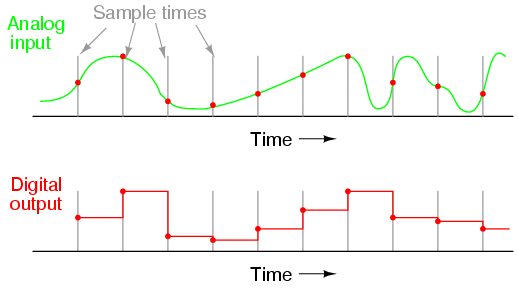
\includegraphics[width=\textwidth]{digitization.png}
                \caption{Analog and Digital signals}
                \label{fig:digitization}
        \end{subfigure}%
        \qquad \quad %add desired spacing between images, e. g. ~, \quad, \qquad etc.
          %(or a blank line to force the subfigure onto a new line)
        \begin{subfigure}[b]{0.5\textwidth}
                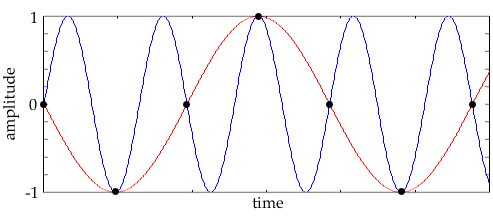
\includegraphics[width=\textwidth]{aliasing.jpg}
                \caption{Aliasing \label{fig:alias} \cite{aliasing}}
                \label{fig:alias}
        \end{subfigure}
        \caption{Digital Conversion \label{fig:digitize}}
\end{figure}

\section{System}
\label{sec:system}
The system simulation model is shown in Figure~\ref{fig:step4}.  As from Step 1, randomly generated bits [Appendix~\ref{app:random_bit_generator}] are converted into symbols [\ref{app:bittosym}] and then upsampled by adding in zeros [\ref{app:impulse_train}].  The result is then is run through a Square Root Raised Cosine (SRRC) pulse shape filter [\ref{app:sqrt_raised_cosine}].  This shaping improves the resistance of the sequence to intersymbol interference (ISI).  The output of this filter is fed into a Digital-to-Analog Converter (DAC).  A DAC takes the digital samples and zero-order holds them at a constant voltage, creating an analog signal [Appendix~\ref{app:da},~\ref{app:zero}].  \\

After the digitizer, a reconstruction filter (also sometimes called an anti-imaging filter) bandlimits the analog waveform output from the DAC.  The high frequency content contained in the stair-case digital signal is undesirable since it can create aliasing of wrongfully high frequency waves.  To avoid this, the Low Pass Filter is used for the reconstruction.  Ours is modeled as a Butterworth filter, or a maximally flat magnitude filter \cite{butter}.  The aim of the filter is to have uniformly flat passband frequency response and roll to zero in the stopband.  As with all filters, the cutoff frequency parameter sets the bands and the order of the filter determines the roll-off of the frequency response in the stopband.  We used a fourth order Butterworth so that the roll-off was $80 \mathtt{\frac{dB}{dec}}$.  We set the cutoff frequency to BLAH BLAH $\mathtt{Hz}$. The interior workings of the filter are not pertinent to this project, so the code in Appendix~\ref{app:butterworth} uses built-in MATLAB functions.  \\

After passing through the reconstruction filter, the analog signal is  sent through a real world channel, modeled by gain and additive white Gaussian noise [Appendix~\ref{app:awgn_channel}].\\

\begin{figure}[H]
\centering
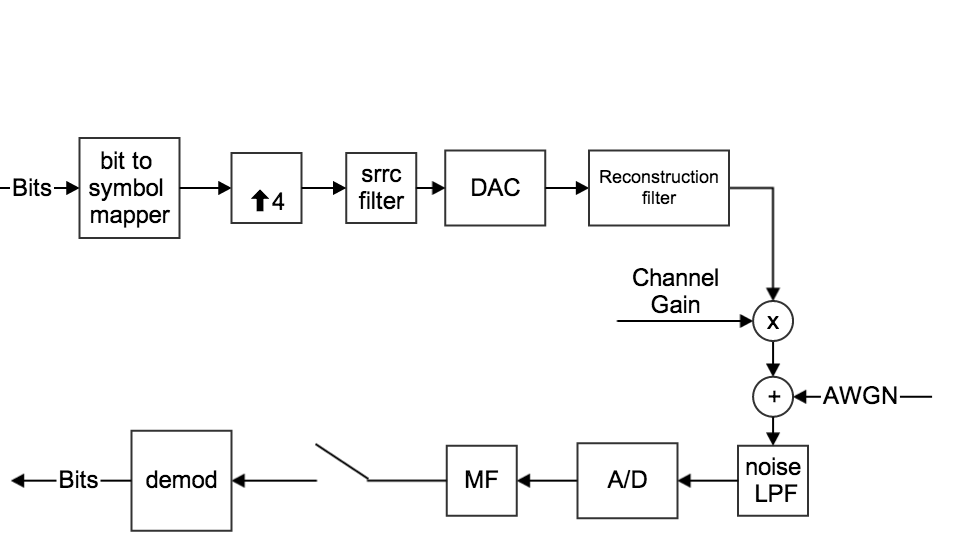
\includegraphics[width=\textwidth]{step4.png}
\caption{Block Diagram of Step 4 system setup\label{fig:step4}}
\end{figure}

To bring the analog back to the digital world, an Analog-to-Digital converter is used [Appendix~\ref{app:ad}].  However, just like before, the conversion is improved by the use of a filter.  An anti-aliasing low-pass filter constrains, or band limits, the channel noise before entering the A/D.  In this setting, the LPF protects against aliasing of high frequency content being recorded at the lower frequency.  We use the same Butterworth filter to accomplish this function.\\

The end of the simulation model is identical to the process in Step 1: a matched filter to the SRRC picks out the symbols from the noisy received signal.  Afterwards, a sampler recovers [Appendix~\ref{app:sampler}] the symbols before a demodulator converts the symbols back into bits [\ref{app:dblocks}].  

\section{Experiments}
\label{sec:experiments}
In this phase of the project, we compare the effect 

\section{Step 4 Results}
\label{sec:results}
In the following sections, the results of the simulations of the different modulation schemes are shown.  For each SER plot, the corresponding results from Step 1 are presented alongside.  The results are interpreted afterwards in the conclusion section.

\begin{figure}[h]
        \centering
        \begin{subfigure}[b]{0.4\textwidth}
                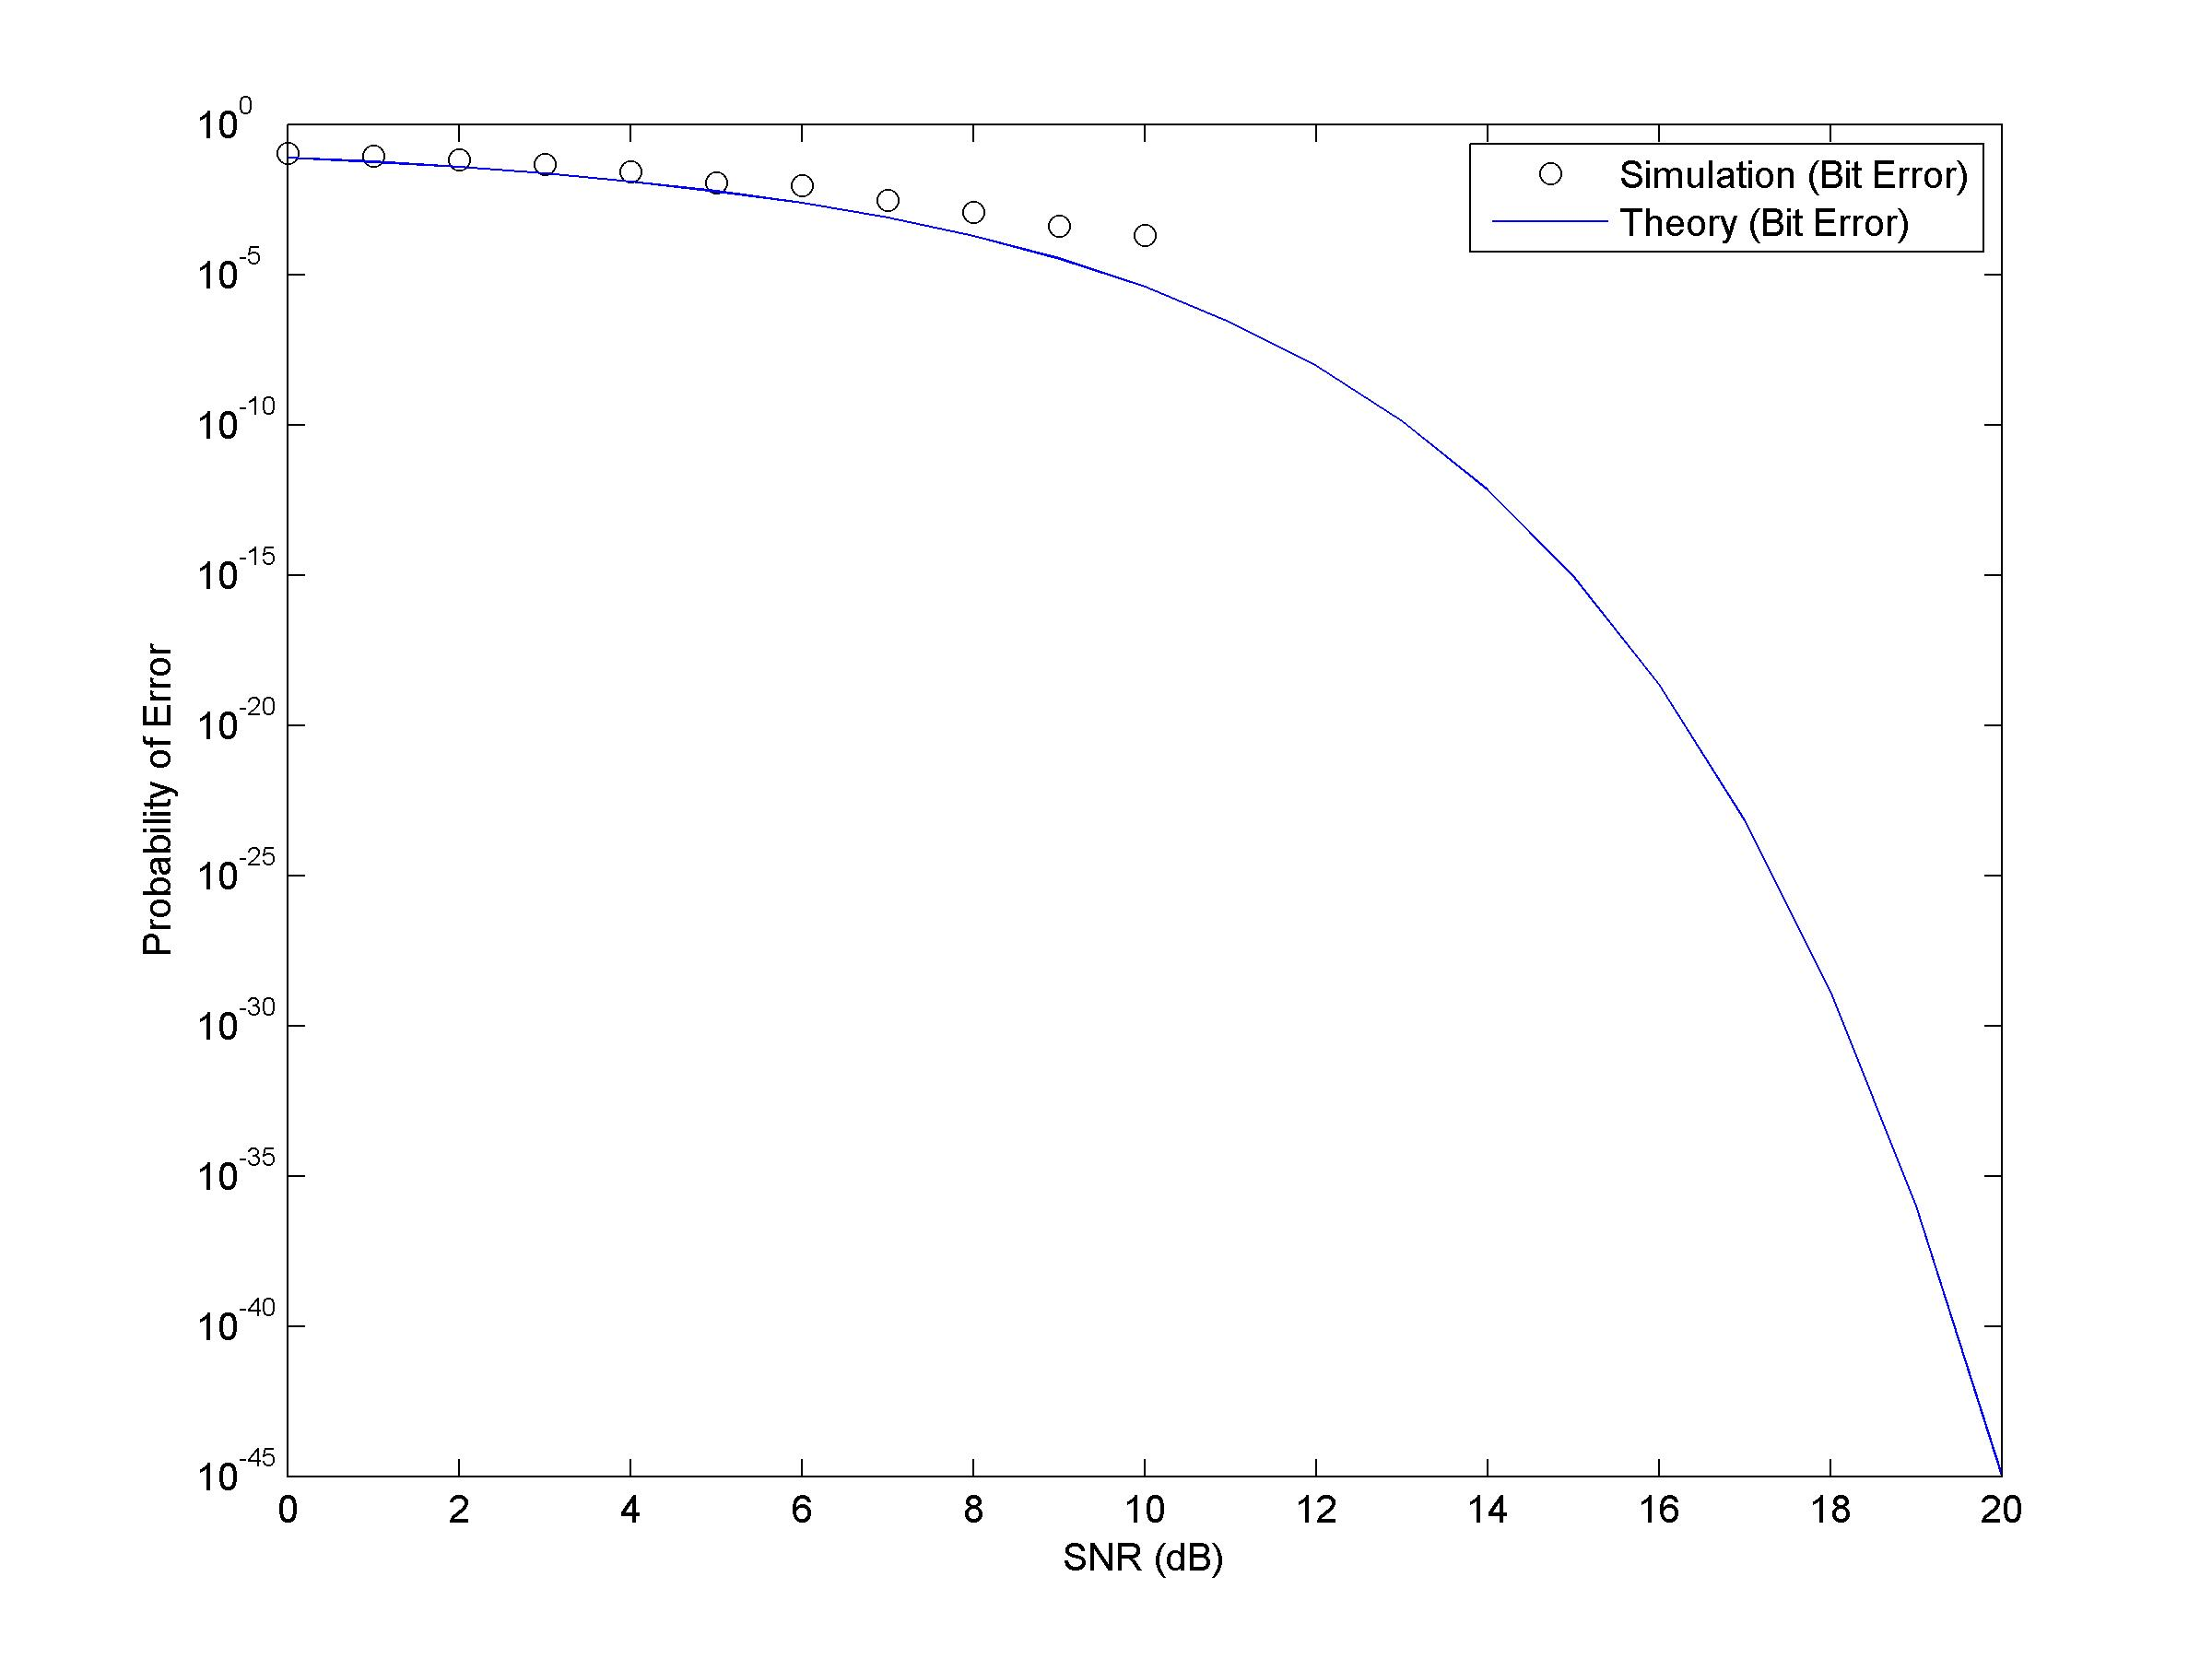
\includegraphics[width=\textwidth]{bpSNR.jpg}
                \caption{Step 4}
                \label{fig:bpSNR}
        \end{subfigure}%
        \qquad \quad %add desired spacing between images, e. g. ~, \quad, \qquad etc.
          %(or a blank line to force the subfigure onto a new line)
        \begin{subfigure}[b]{0.4\textwidth}
                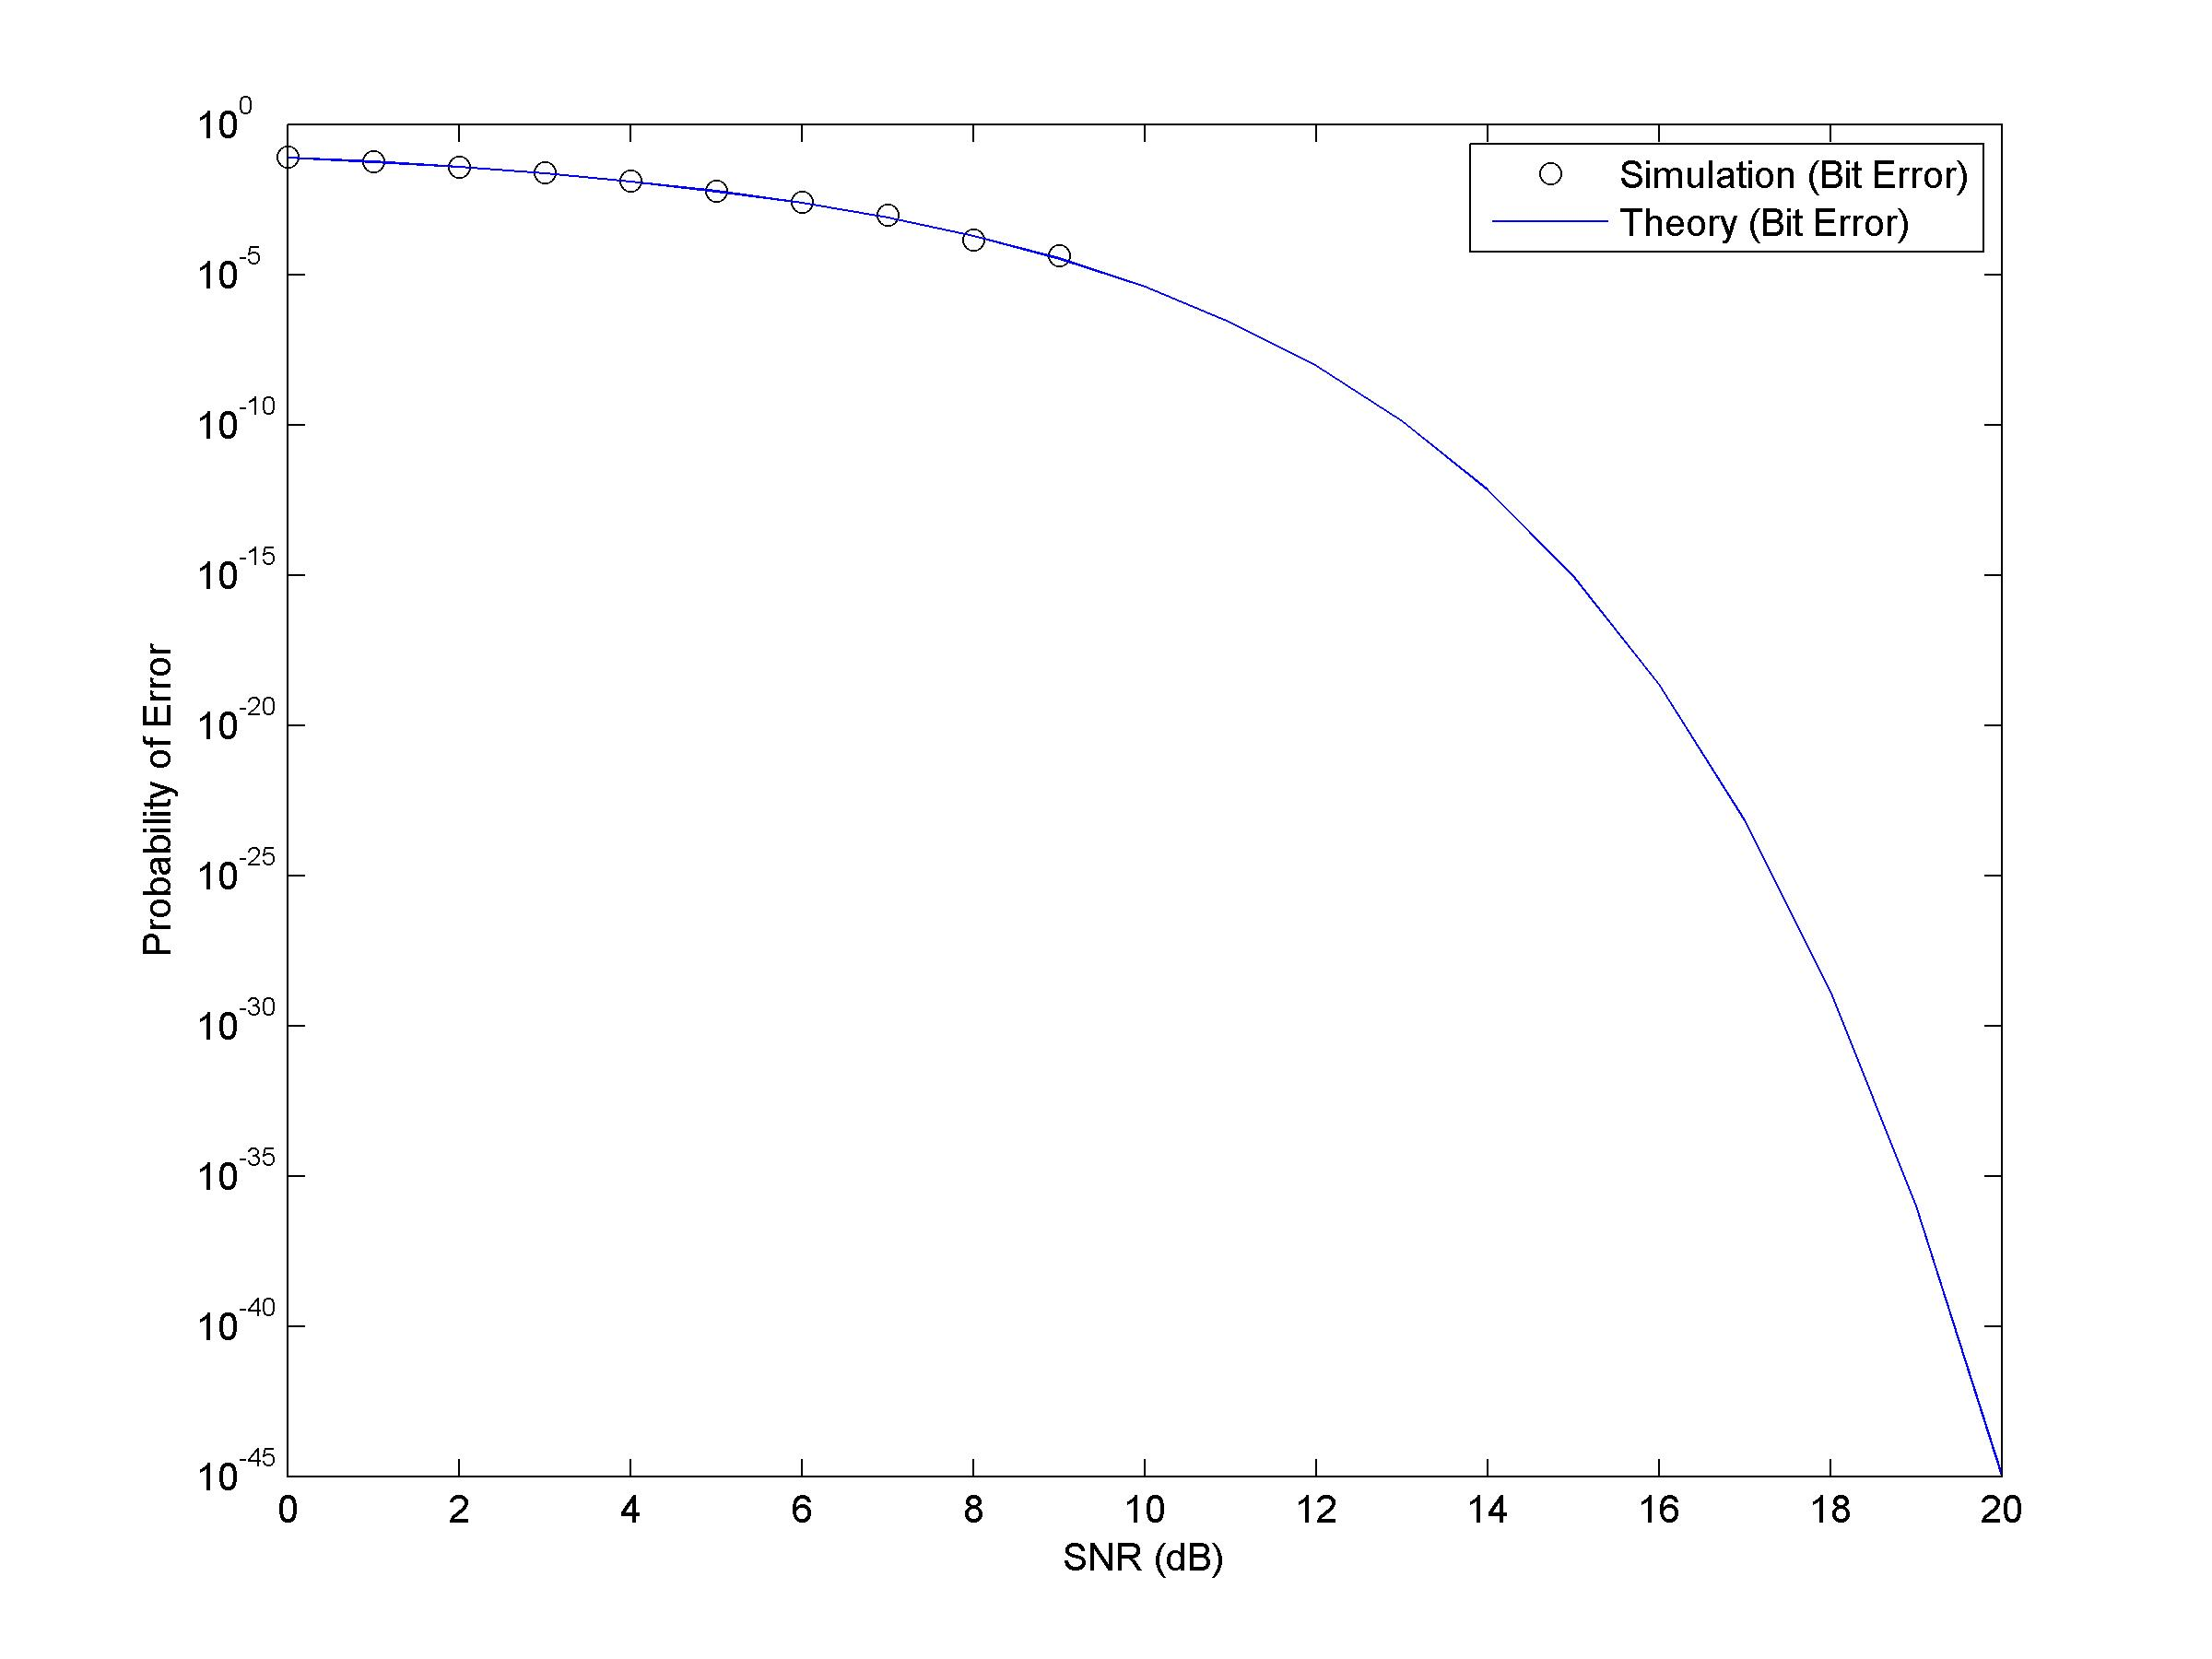
\includegraphics[width=\textwidth]{bpSNRstep1.jpg}
                \caption{Step 1}
                \label{fig:bpSNR1}
        \end{subfigure}
        \caption{BPSK Symbol Error Rate Comparison \label{fig:bpsk}}
\end{figure}

\begin{figure}[h]
        \centering
        \begin{subfigure}[b]{0.4\textwidth}
                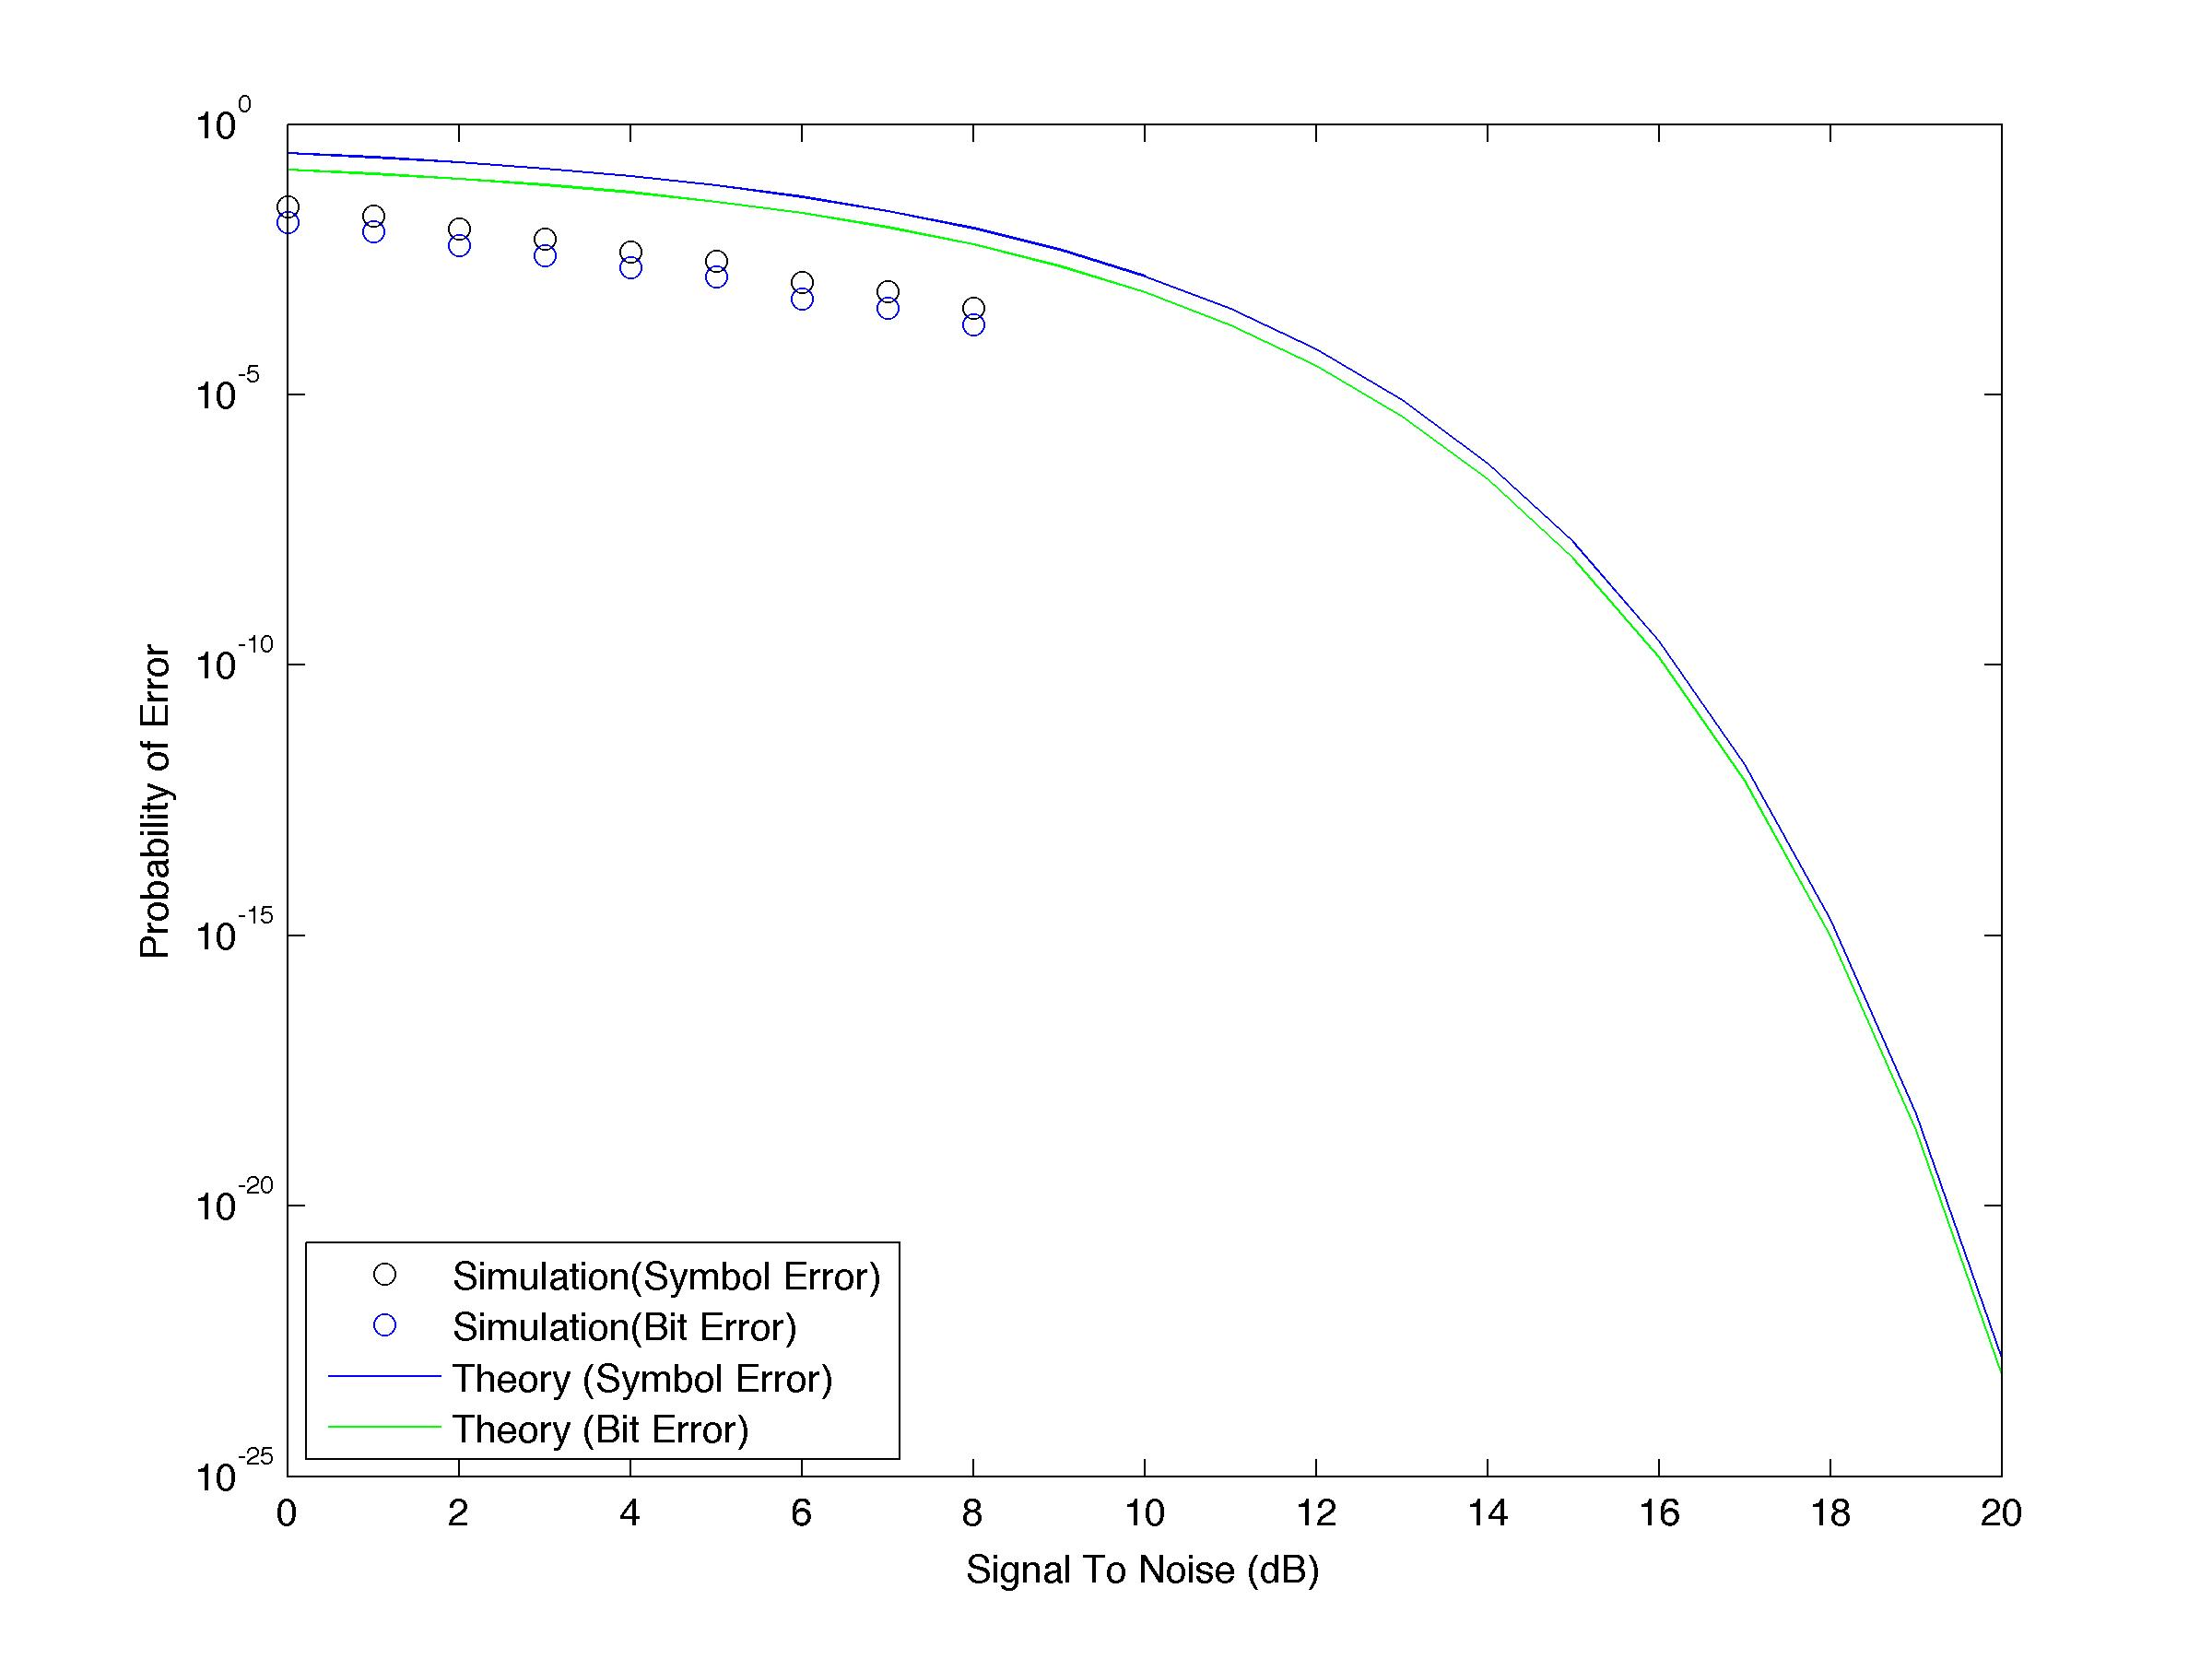
\includegraphics[width=\textwidth]{qpSNR.jpg}
                \caption{Step 4}
                \label{fig:pqSNR}
        \end{subfigure}%
        \qquad \quad %add desired spacing between images, e. g. ~, \quad, \qquad etc.
          %(or a blank line to force the subfigure onto a new line)
        \begin{subfigure}[b]{0.4\textwidth}
                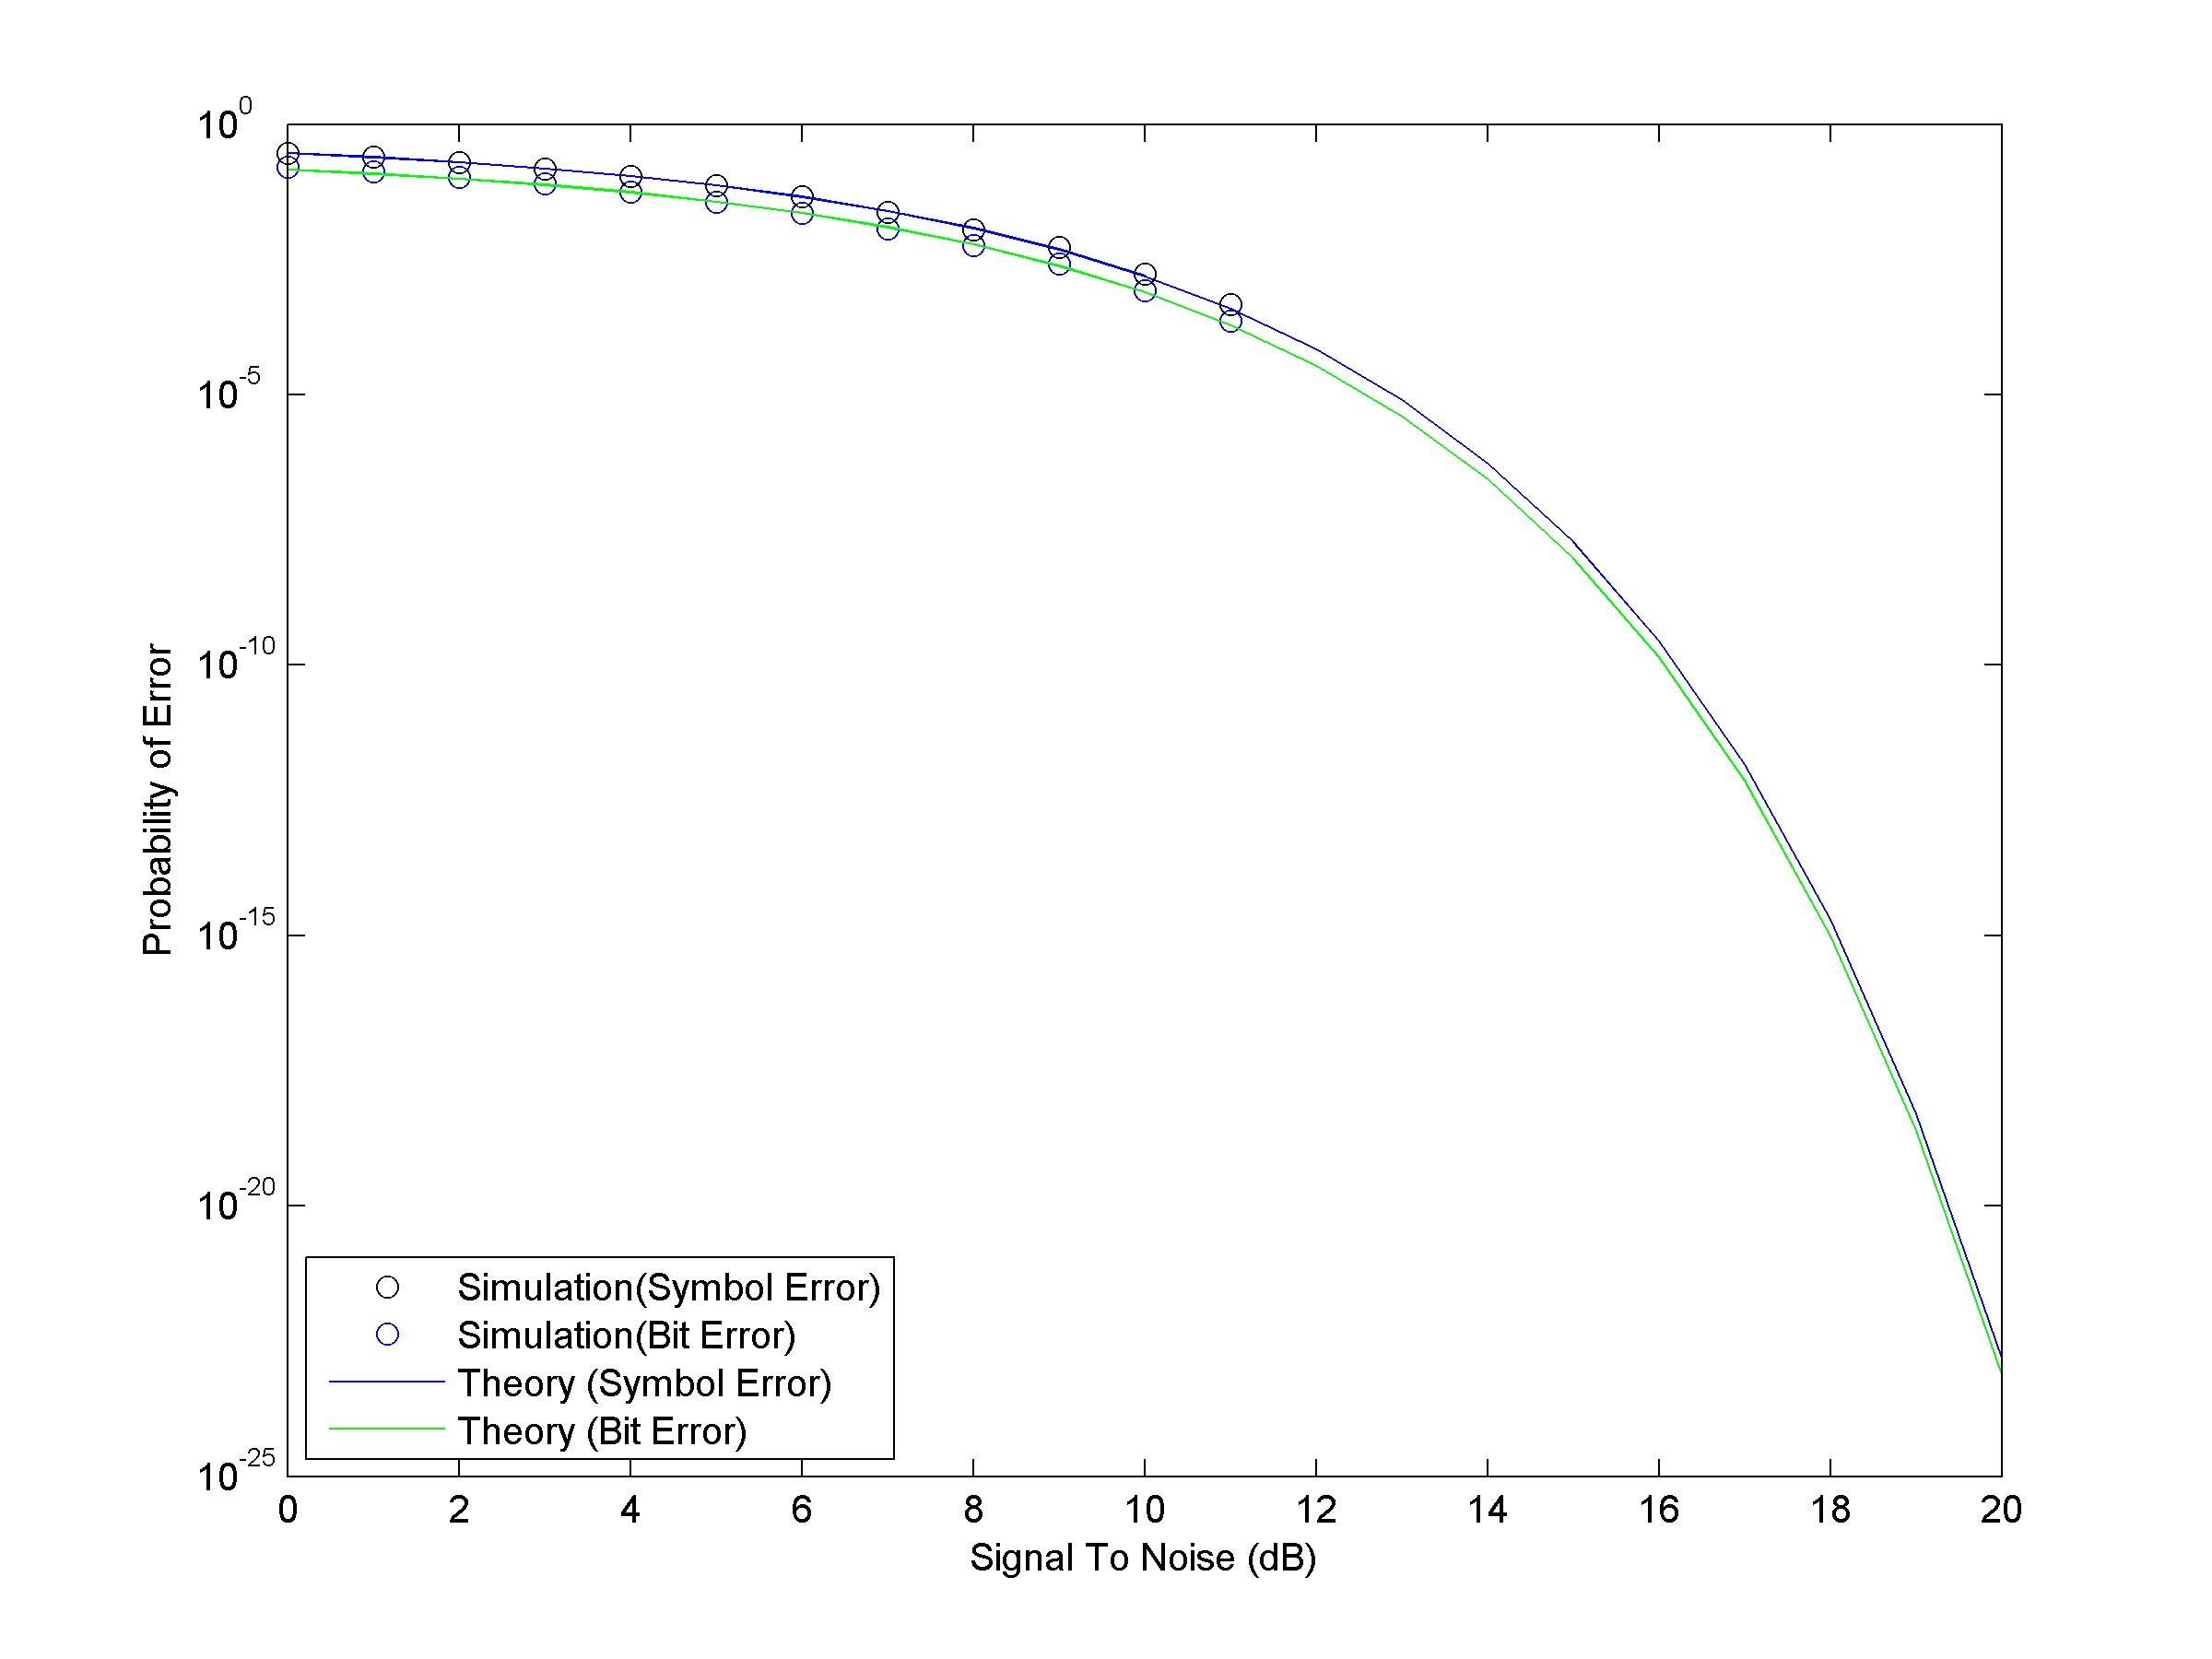
\includegraphics[width=\textwidth]{qpSNRstep1.jpg}
                \caption{Step 1}
                \label{fig:qpSNR1}
        \end{subfigure}
        \caption{QPSK Bit Error Rate Comparison \label{fig:qpsk}}
\end{figure}

\begin{figure}[h]
        \centering
        \begin{subfigure}[b]{0.4\textwidth}
                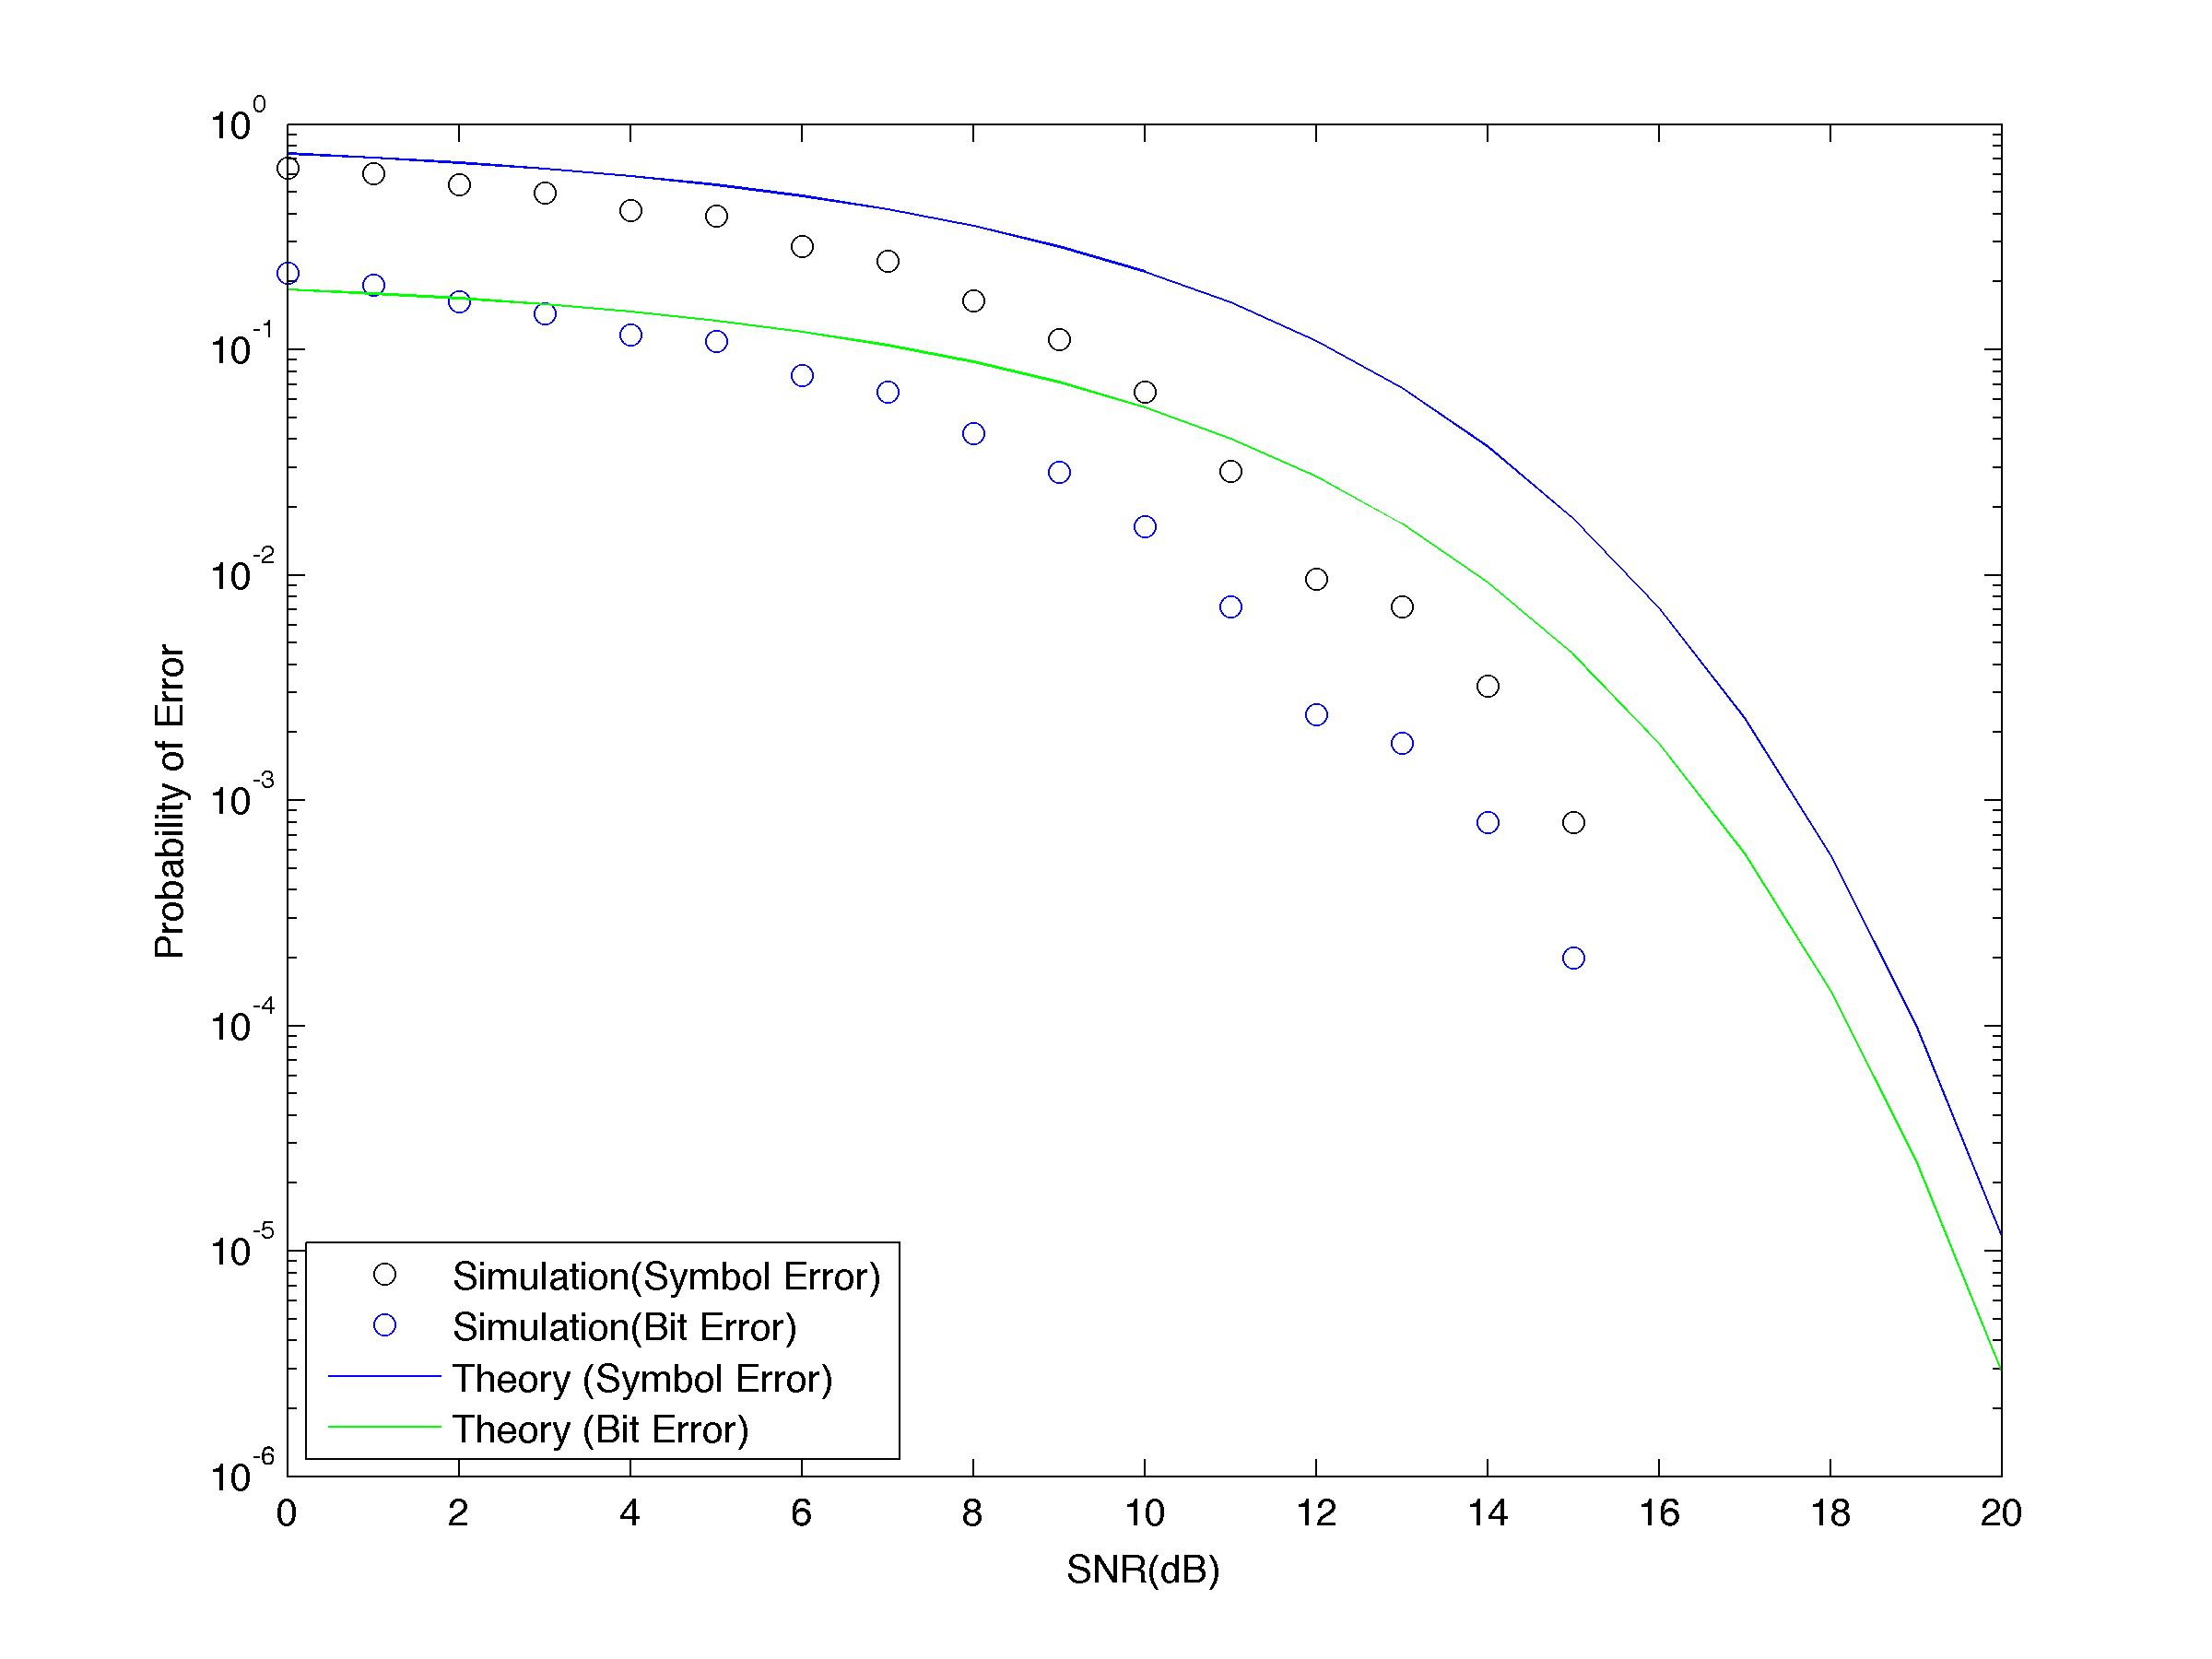
\includegraphics[width=\textwidth]{qam16SNR.jpg}
                \caption{Step 4}
                \label{fig:bpSNR}
        \end{subfigure}%
        \qquad \quad %add desired spacing between images, e. g. ~, \quad, \qquad etc.
          %(or a blank line to force the subfigure onto a new line)
        \begin{subfigure}[b]{0.4\textwidth}
                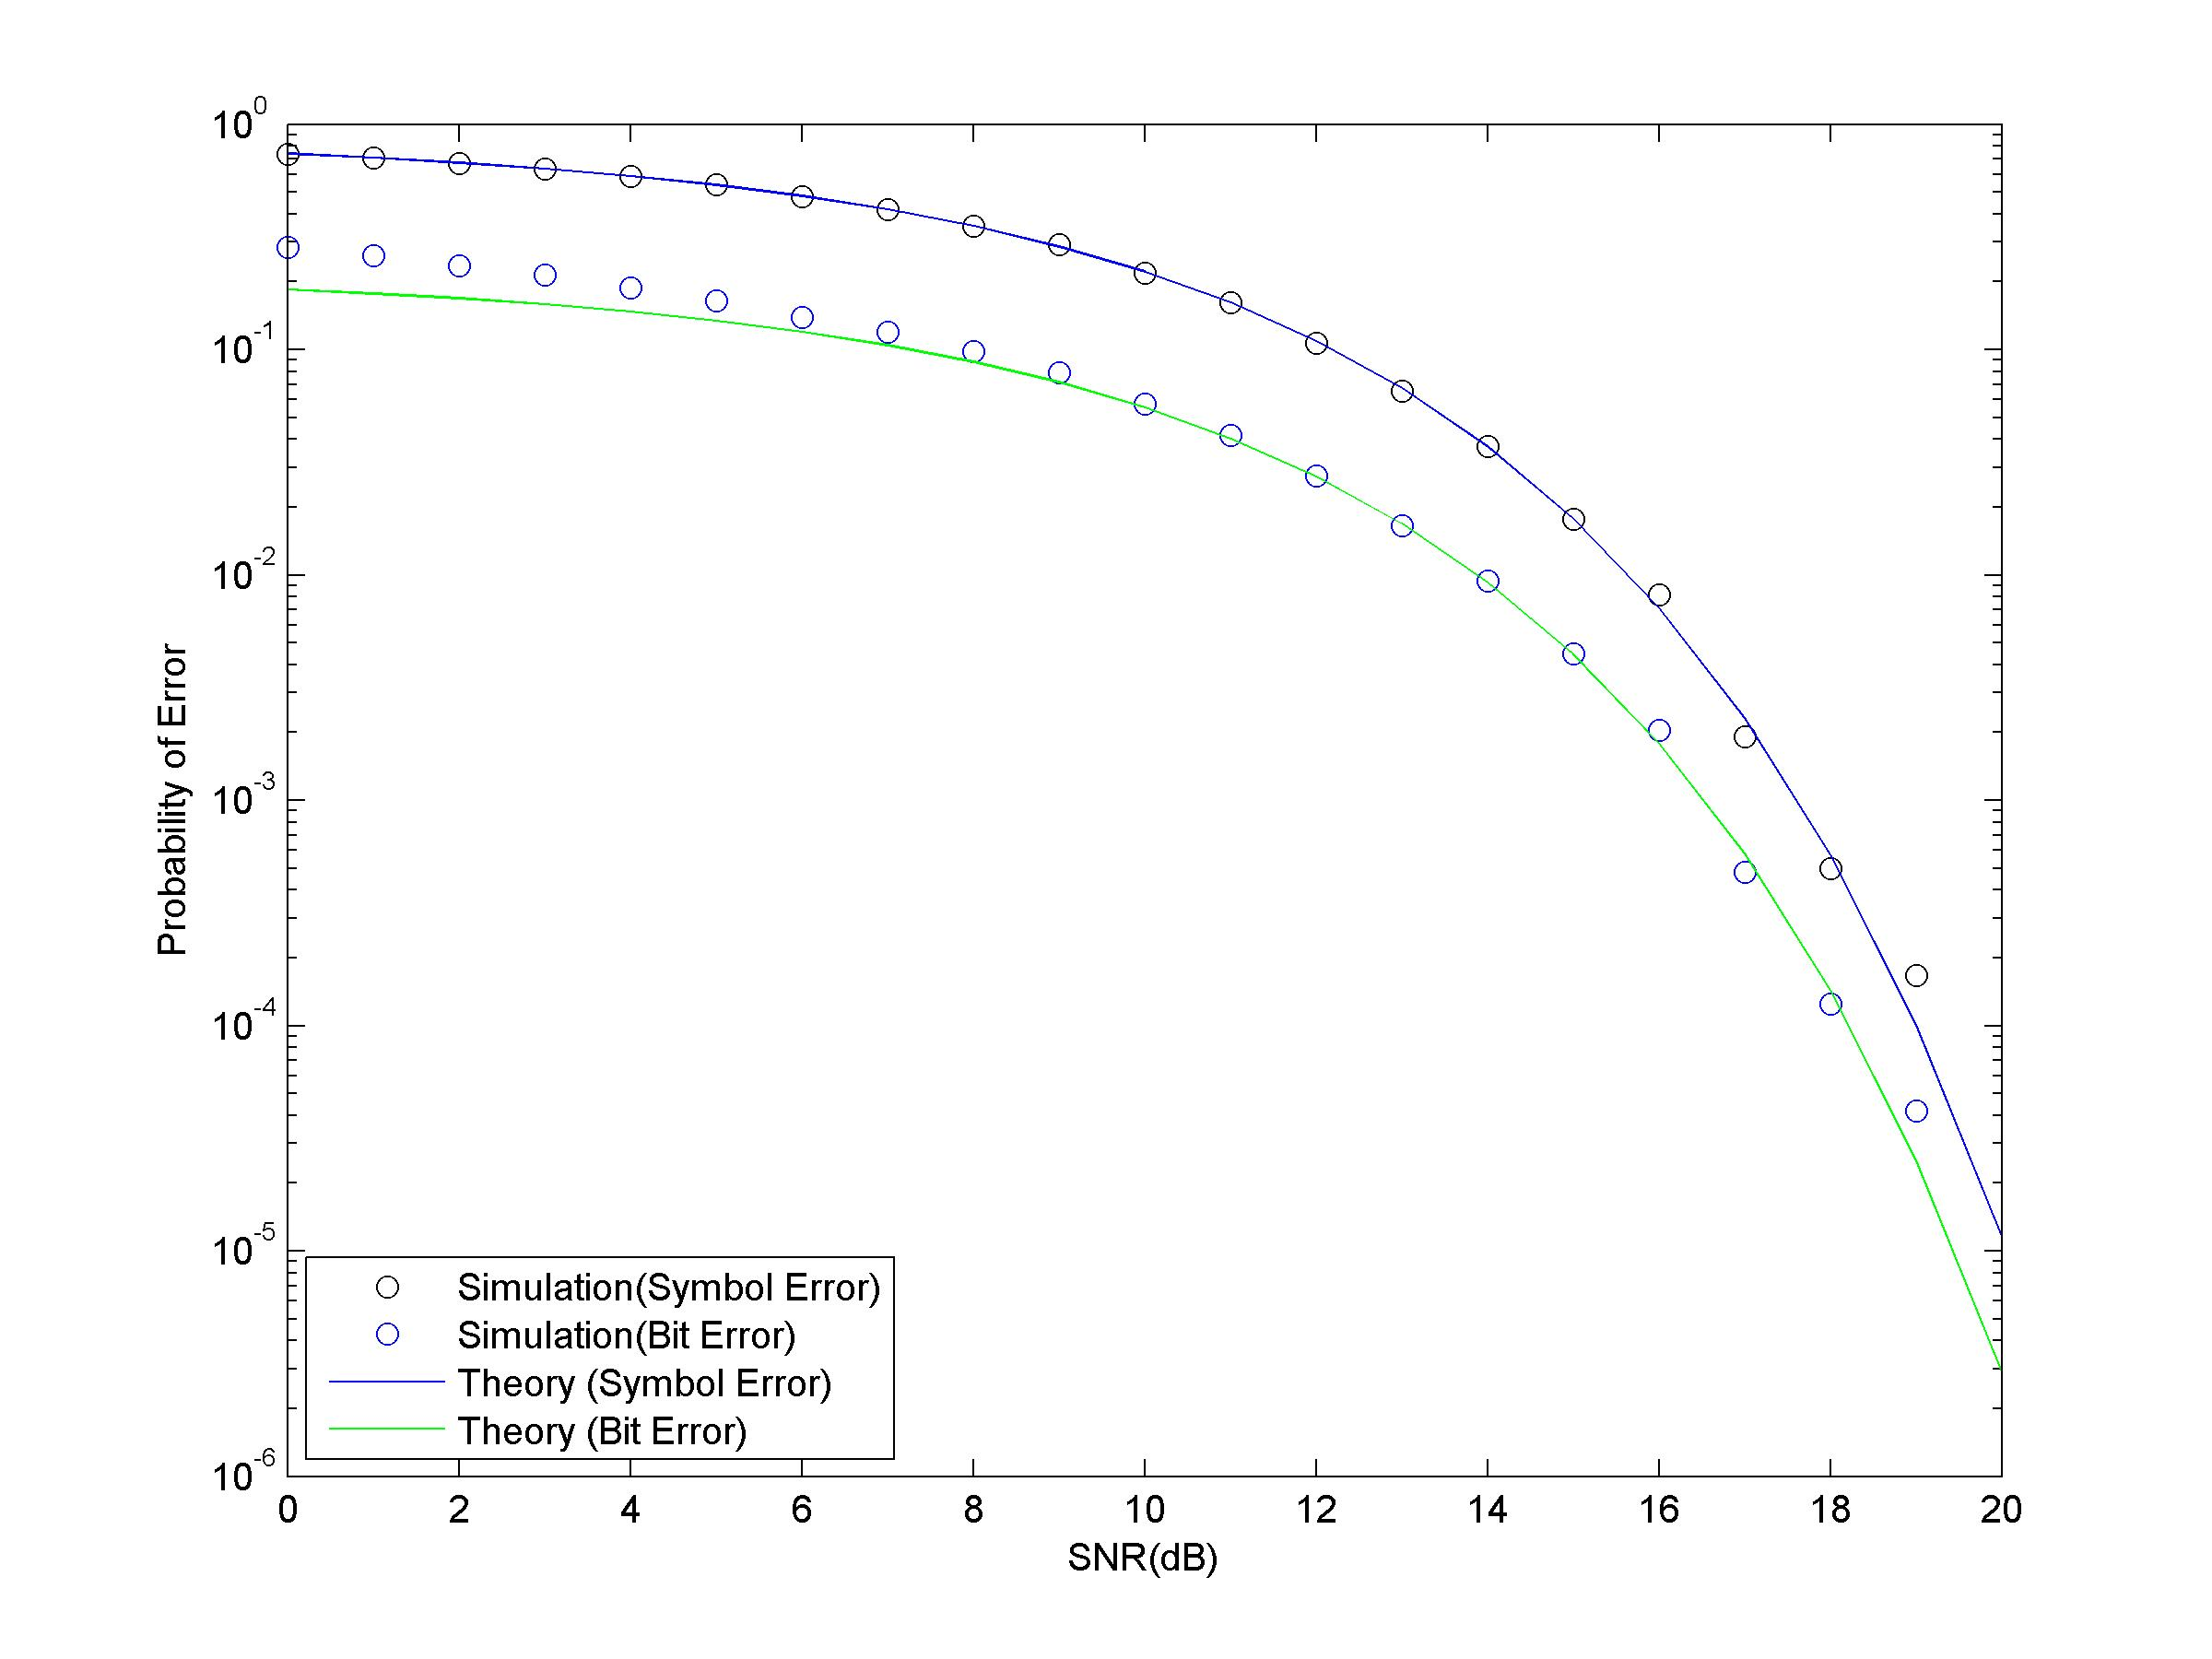
\includegraphics[width=\textwidth]{qam16SNRstep1.jpg}
                \caption{Step 1}
                \label{fig:bpSNR1}
        \end{subfigure}
        \caption{16-QAM Bit Error Rate Comparison \label{fig:qam16}}
\end{figure}

\begin{figure}[h]
        \centering
        \begin{subfigure}[b]{0.4\textwidth}
                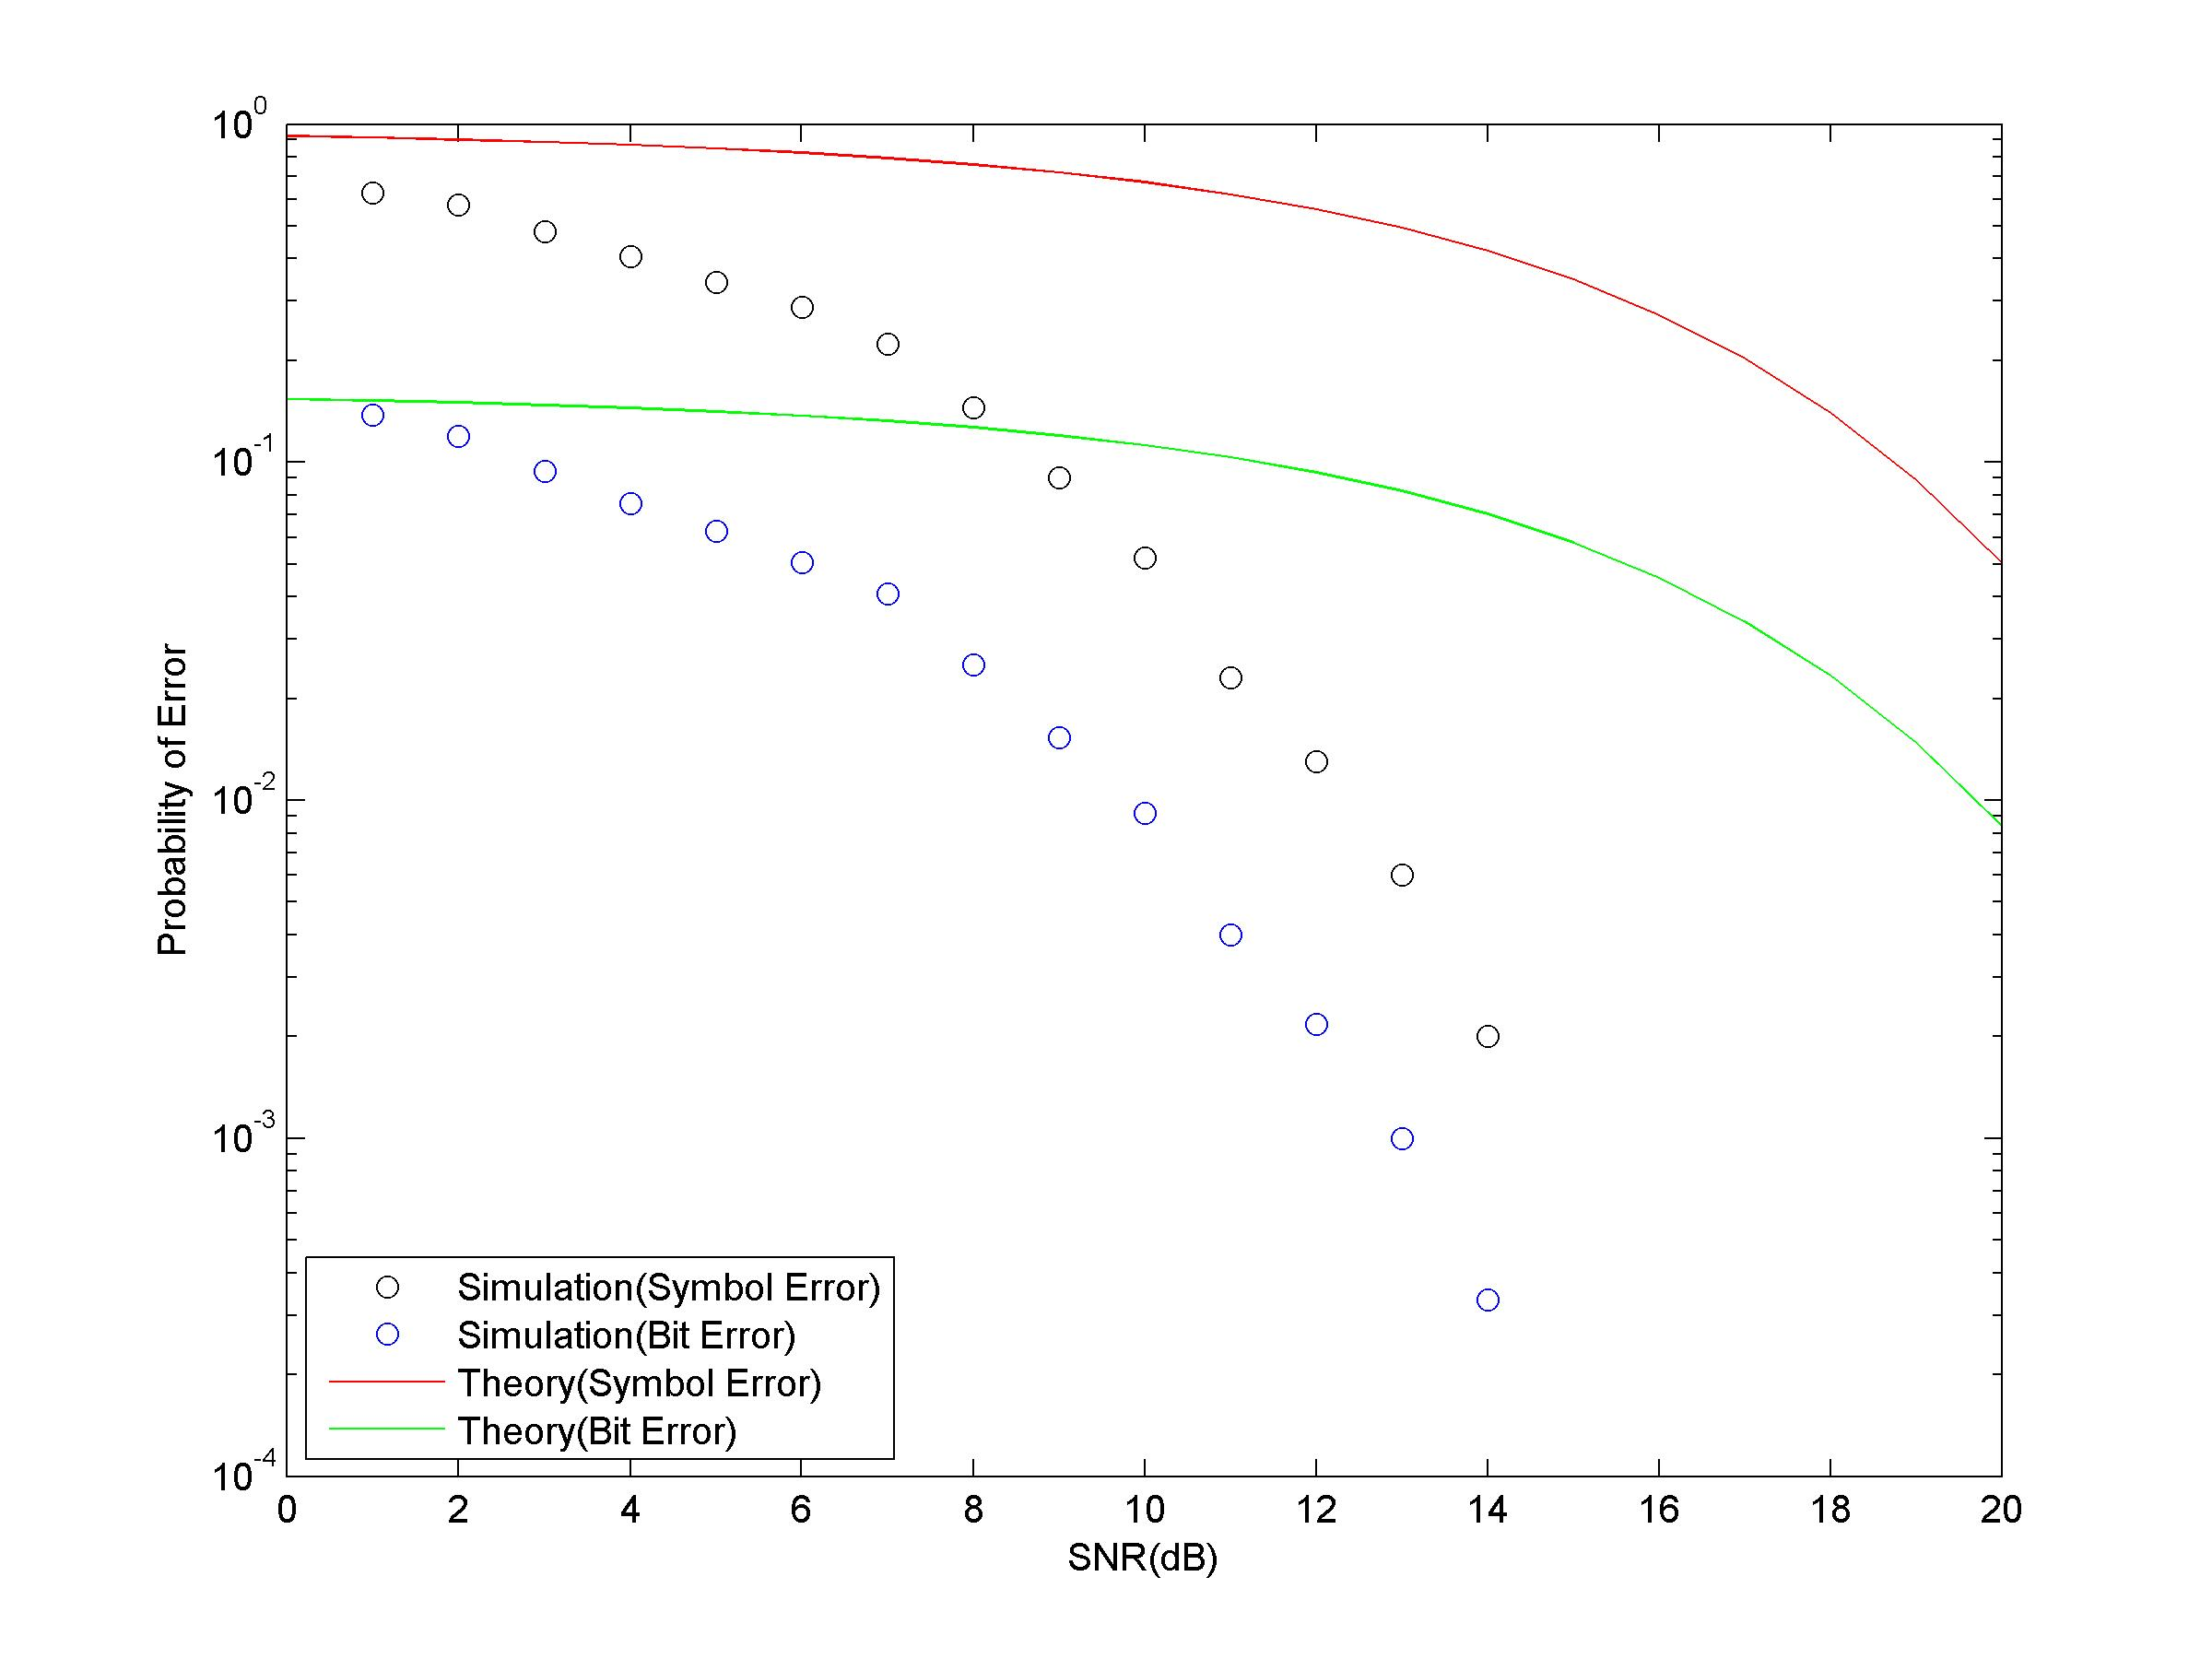
\includegraphics[width=\textwidth]{qam64SNR.jpg}
                \caption{Step 4}
                \label{fig:bpSNR}
        \end{subfigure}%
        \qquad \quad %add desired spacing between images, e. g. ~, \quad, \qquad etc.
          %(or a blank line to force the subfigure onto a new line)
        \begin{subfigure}[b]{0.4\textwidth}
                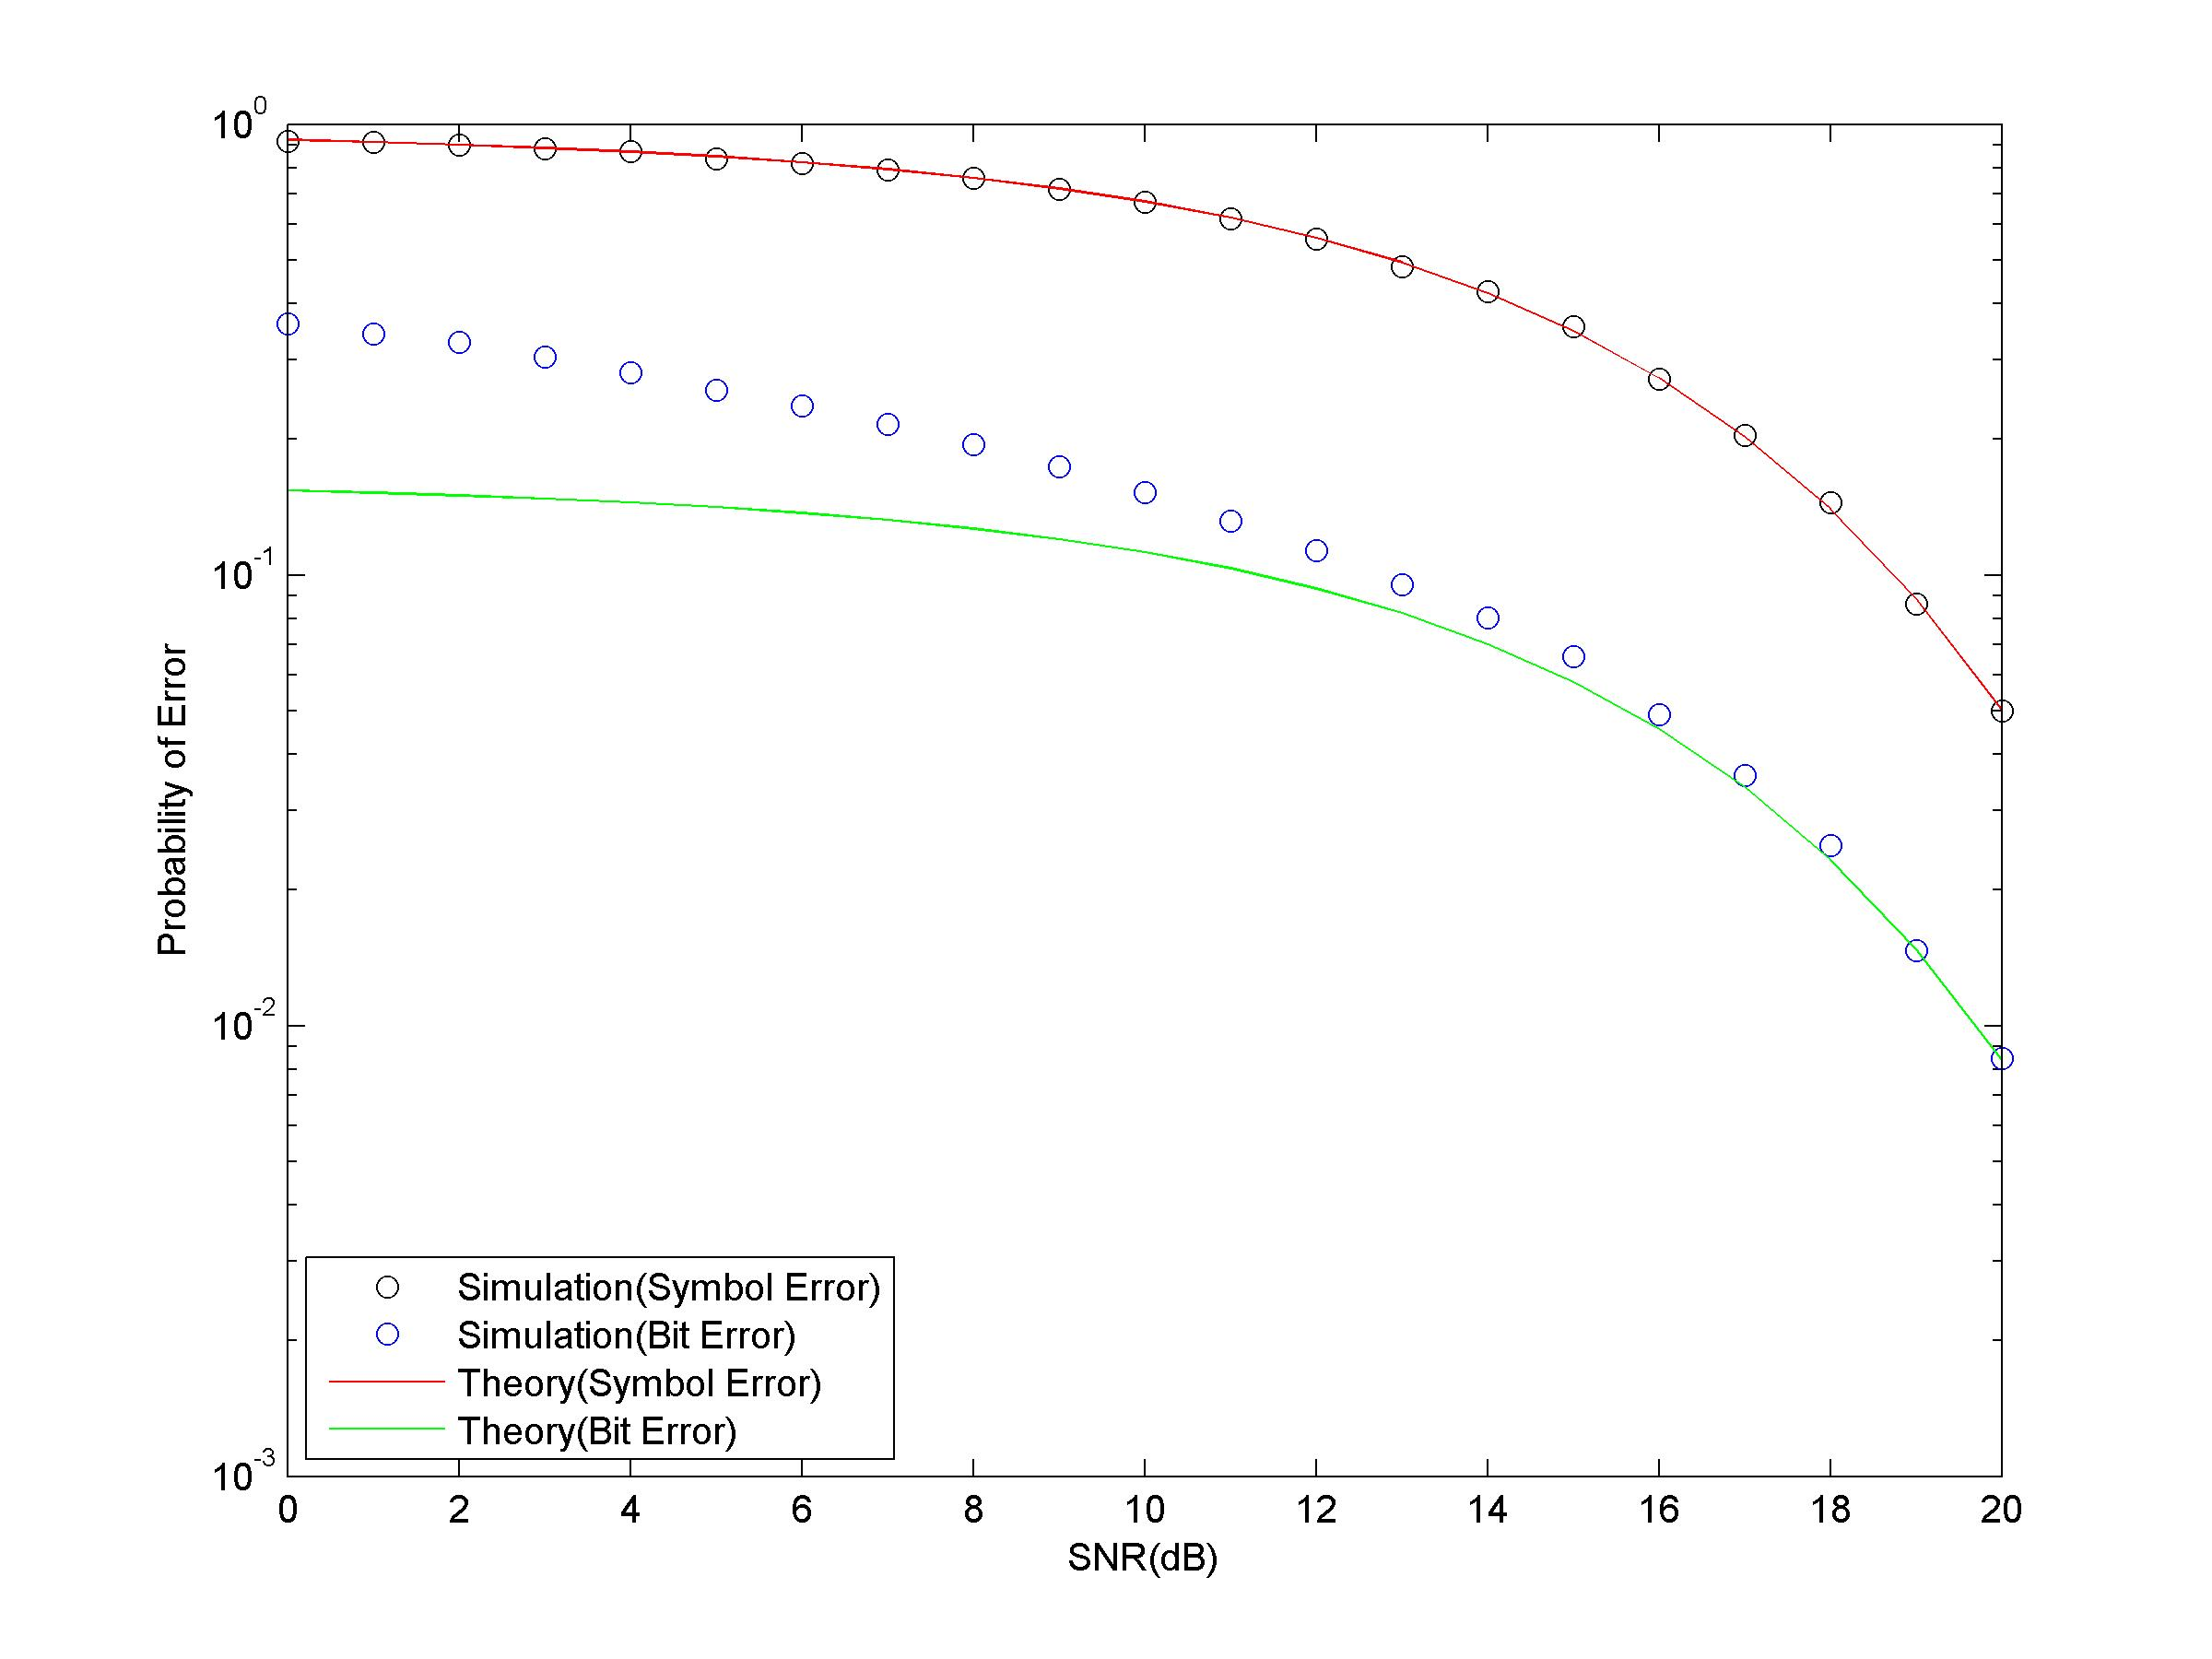
\includegraphics[width=\textwidth]{qam64SNRstep1.jpg}
                \caption{Step 1}
                \label{fig:bpSNR1}
        \end{subfigure}
        \caption{64-QAM Symbol Error Rate Comparison \label{fig:qam64}}
\end{figure}


%
%\subsubsection{Constellation Plots  for Phase Recovery}
%\begin{figure}[H]
%\centering
%\hspace*{-2cm}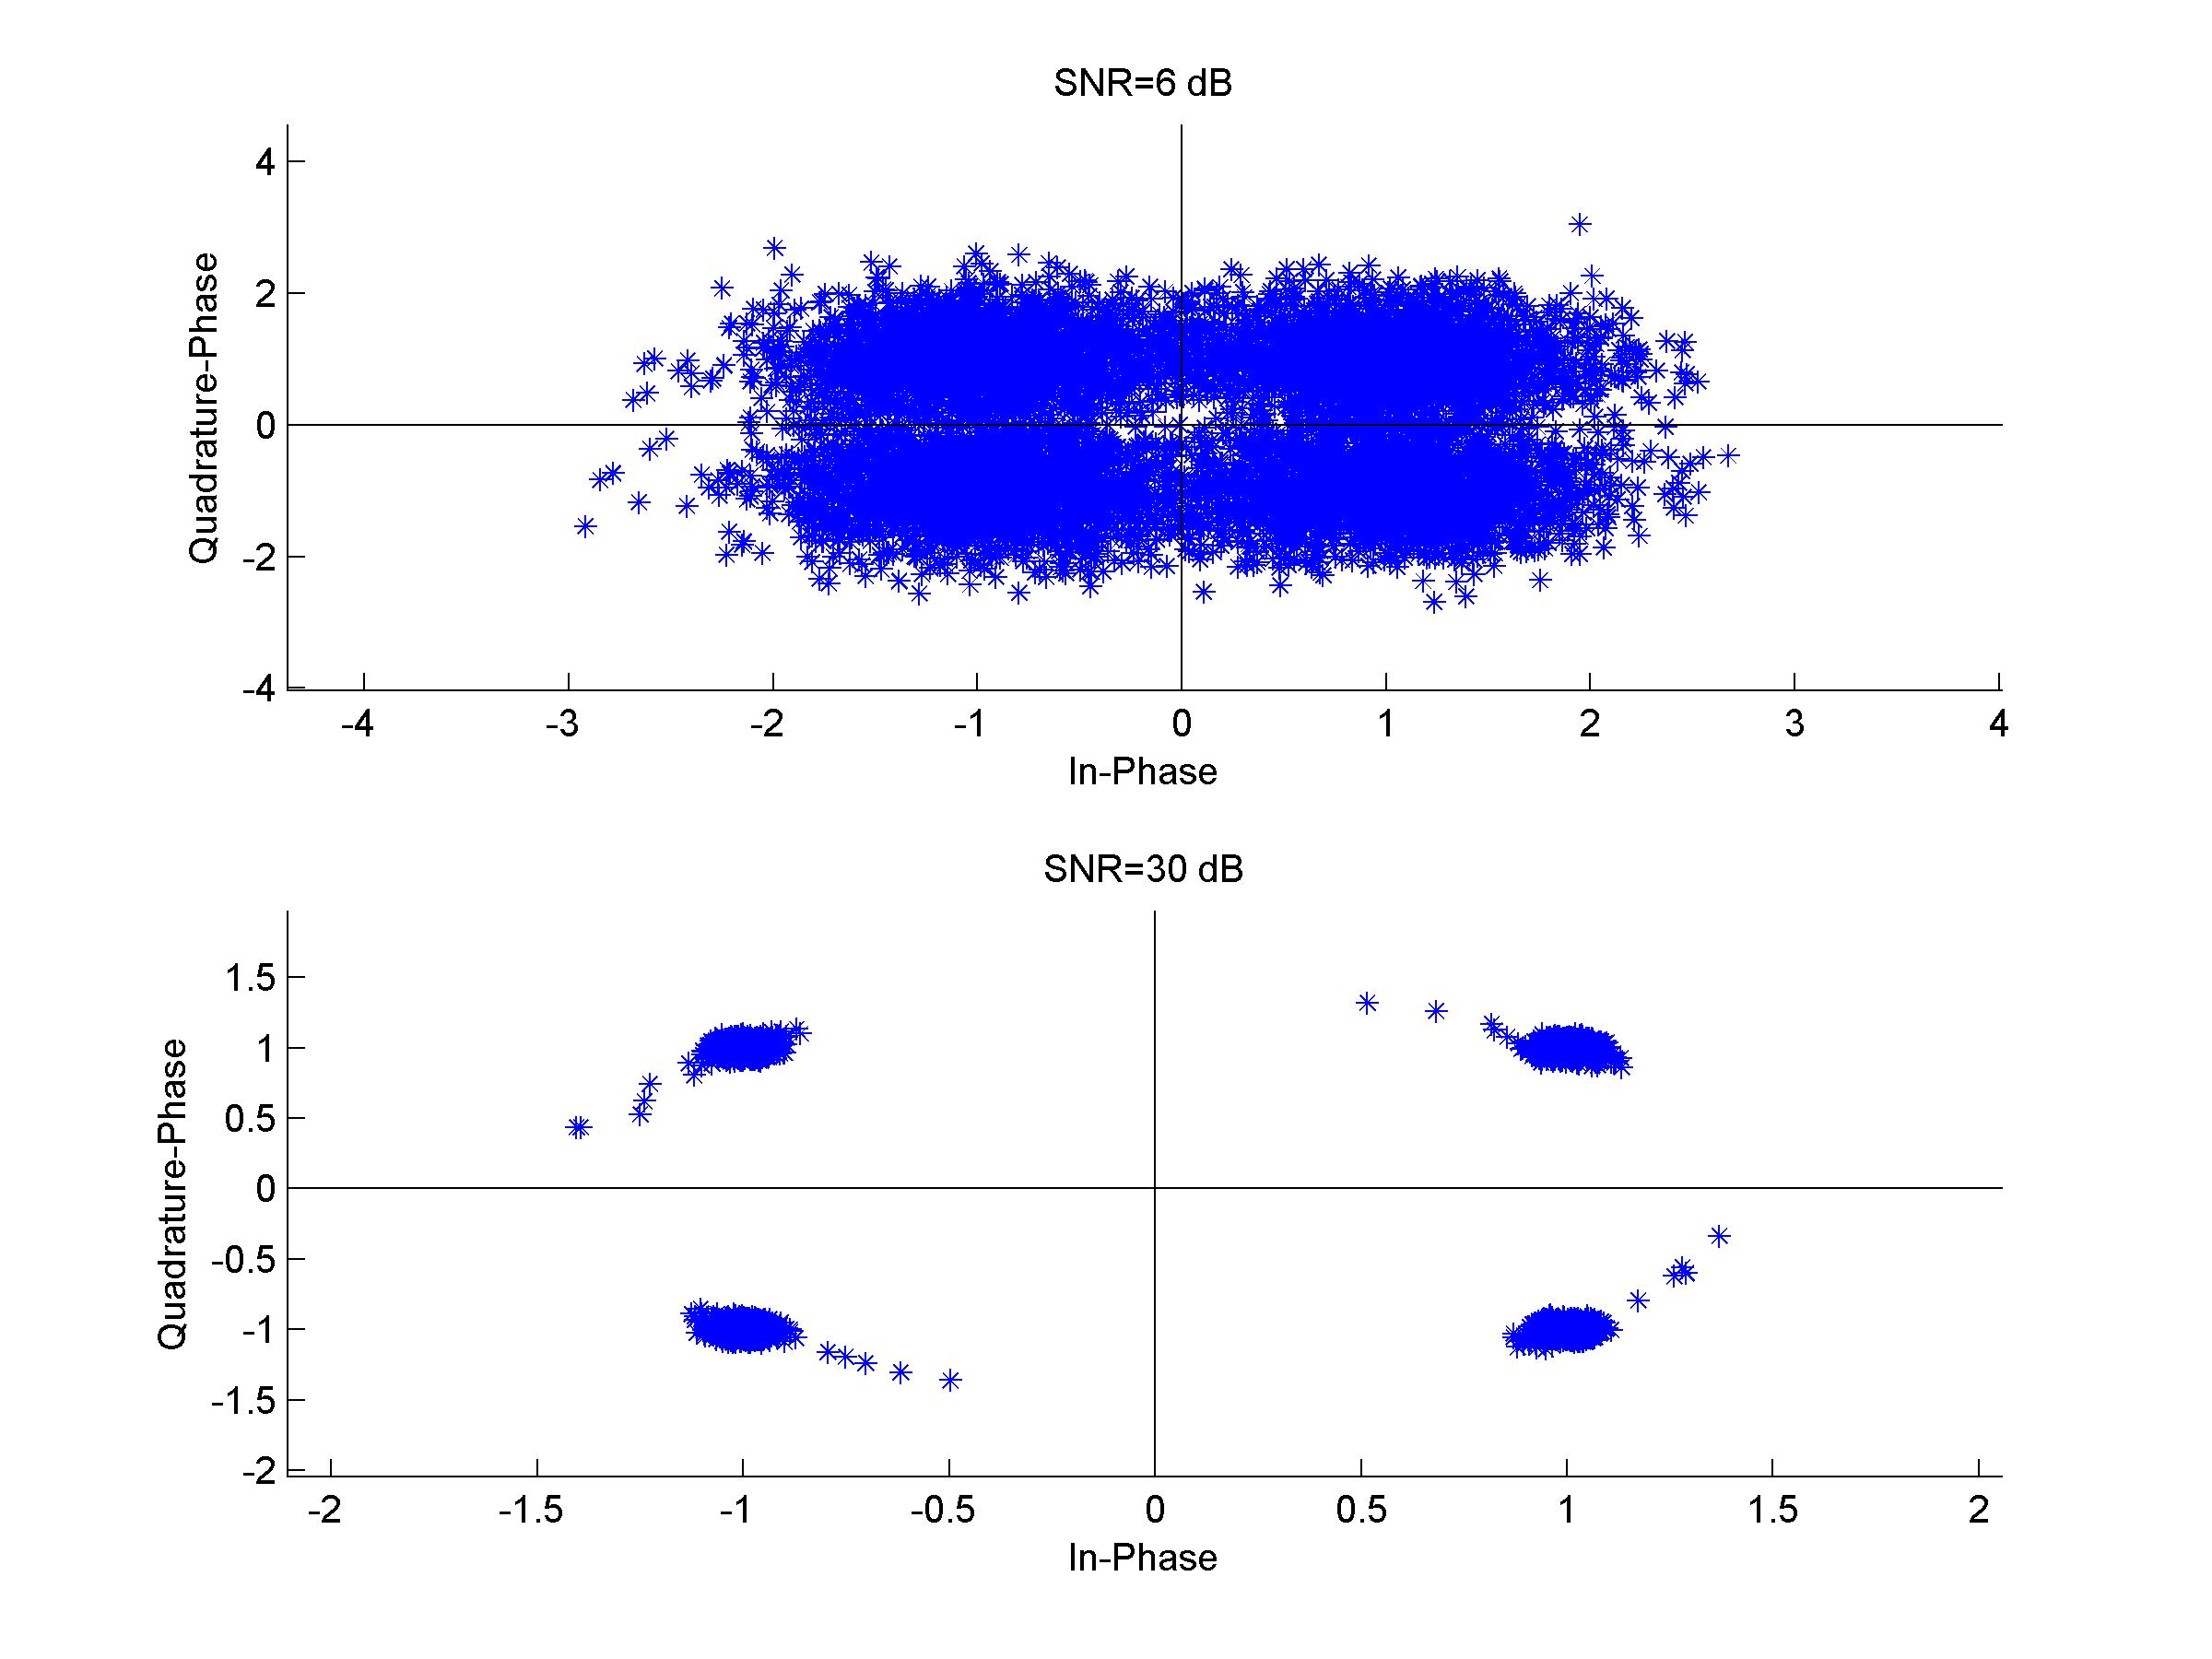
\includegraphics[width=0.7\textwidth]{qpConstpo_ddr1.jpg}
%\caption{The resulting constellation plot of the output of the system with Decision Directed Recovery Loop for an input with 30 degrees phase offset at 6dB and 30dB SNR \label{fig:ddrConstPhase}}
%\end{figure}
%
%\subsubsection{BER Plots for Phase Recovery}
%\begin{figure}[H]
%\centering
%\hspace*{-2cm}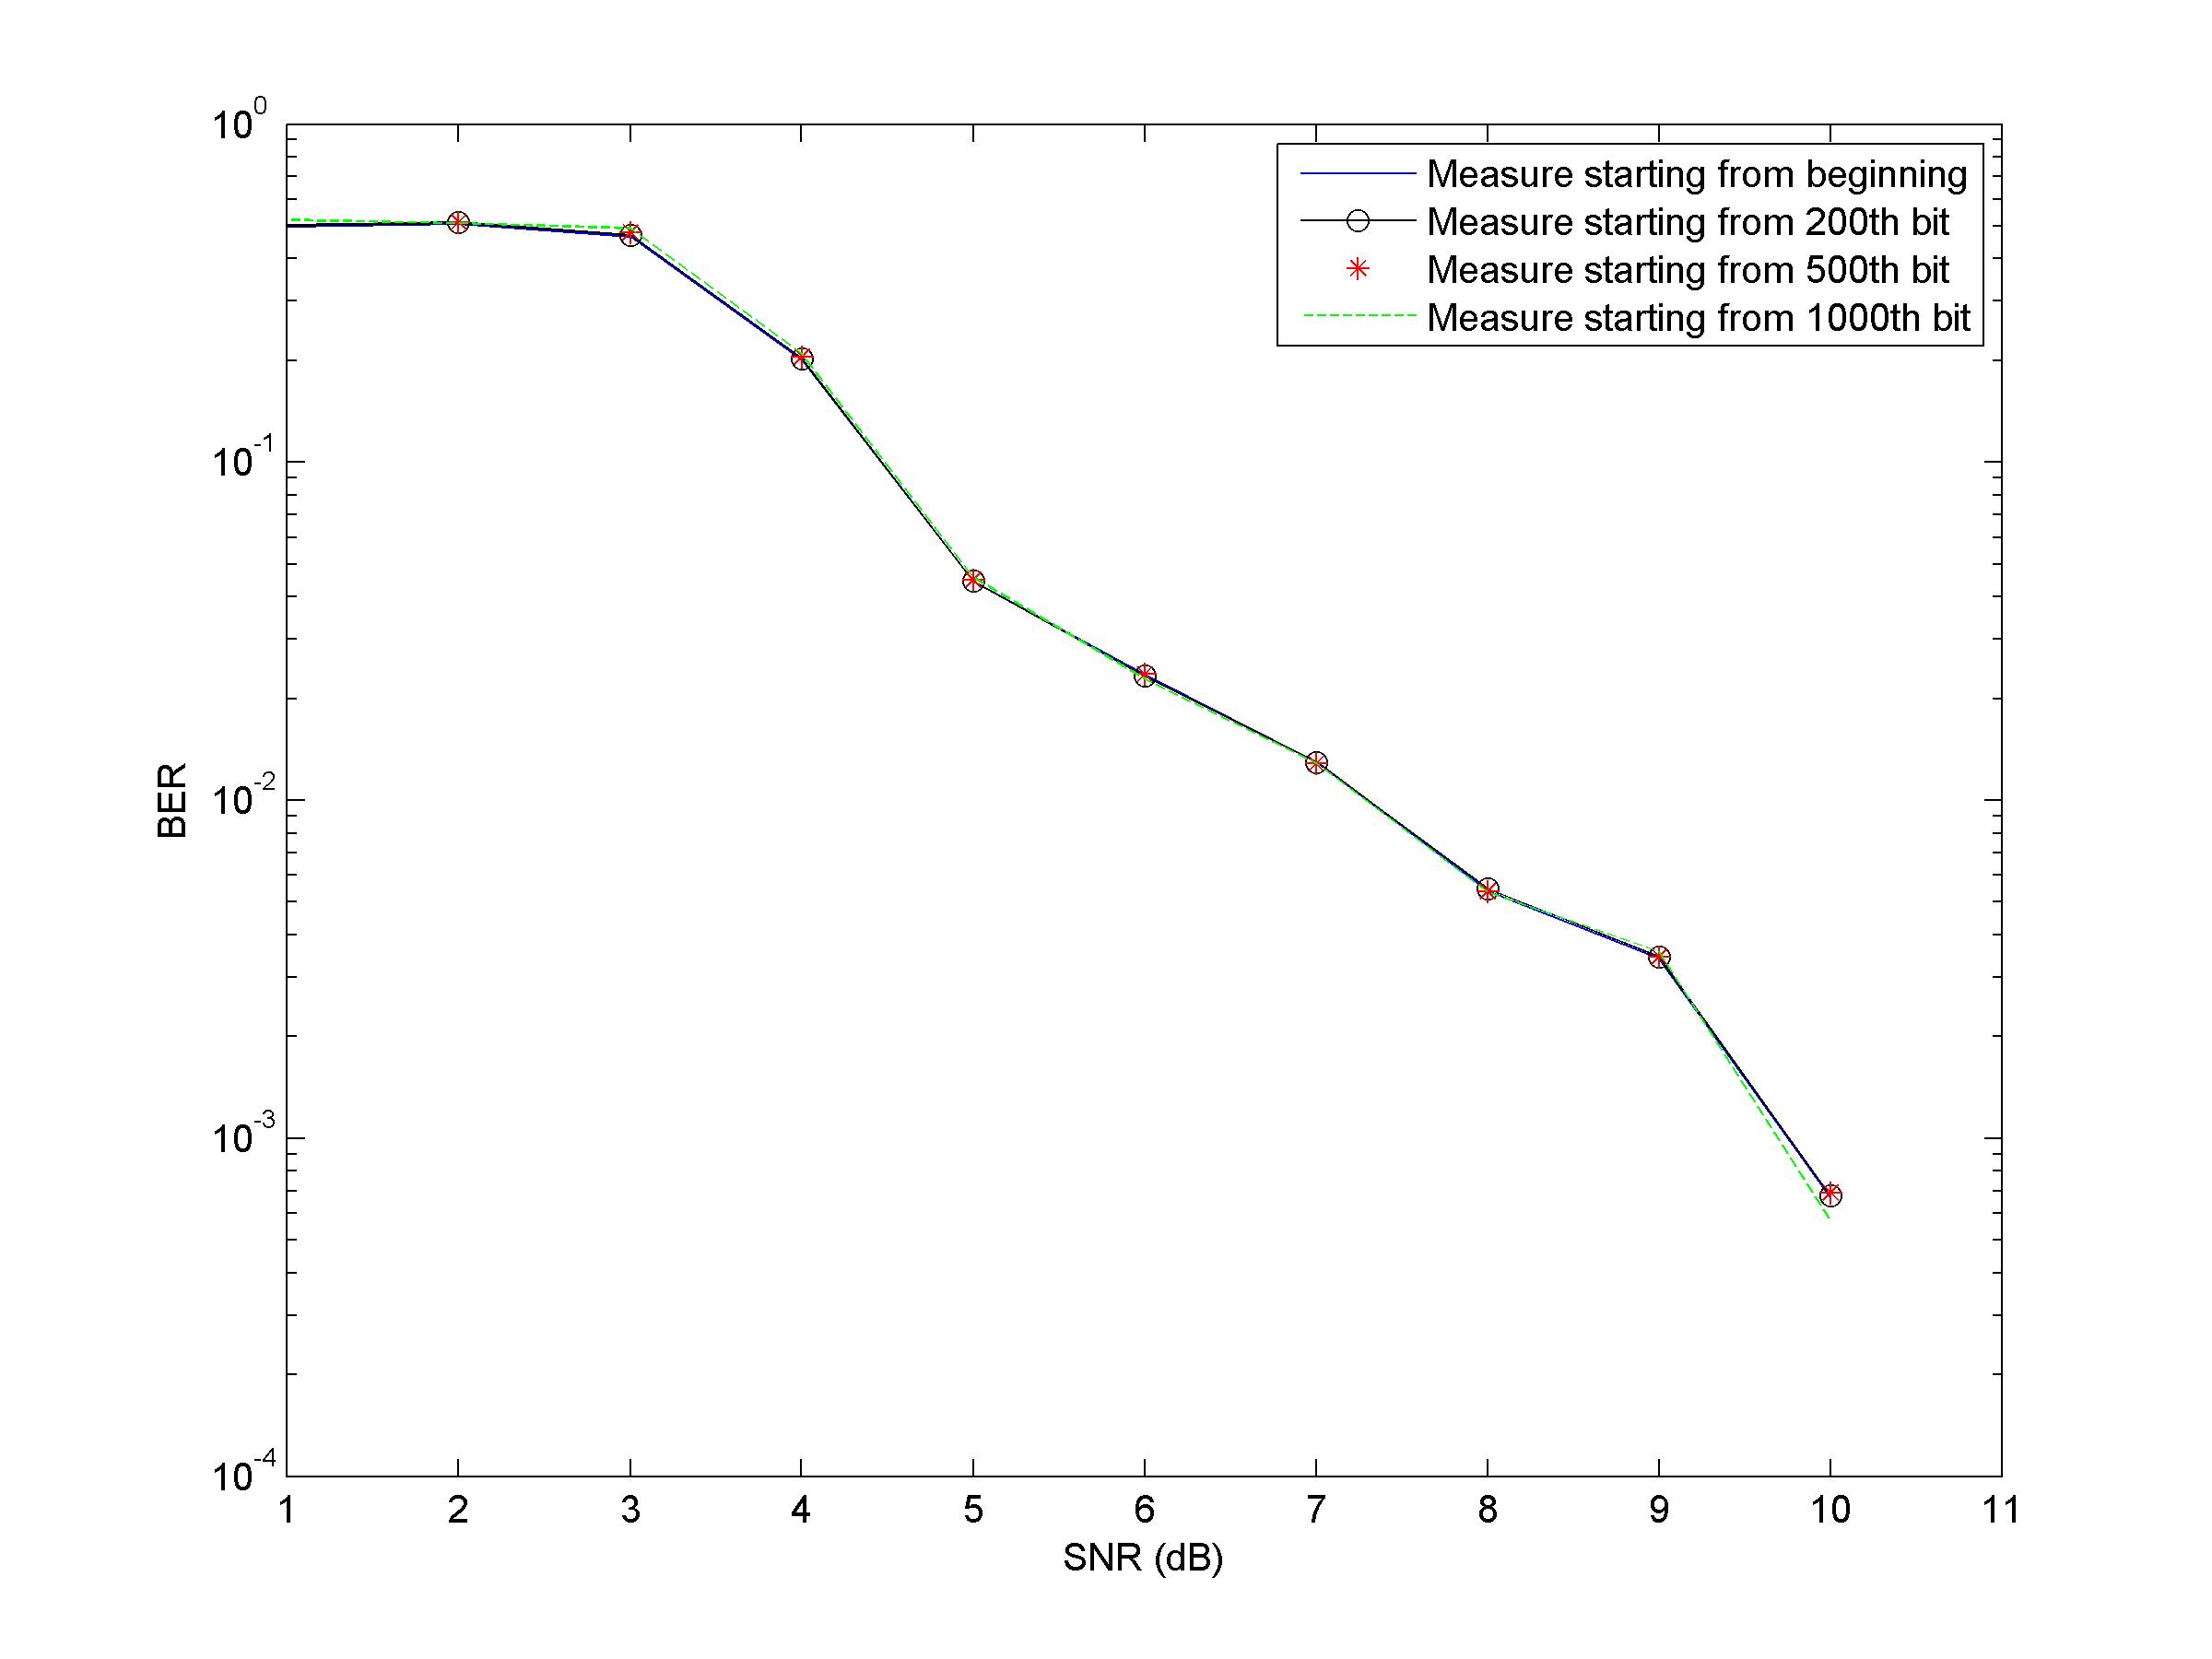
\includegraphics[width=0.7\textwidth]{qpBERpo_ddr1.jpg}
%\caption{BER plots of the system with Decision Directed Recovery Loop for an input with 30 degrees phase offset (using output bits starting from different indexes) \label{fig:ddrBERphase}}
%\end{figure}
%
%\subsubsection{BER Plots for Carrier Recovery}



\newpage
\section{Conclusion}
\label{sec:conc}

The objective of this step was to visualize the effects of data converters in the system model.  Analog and digital waveforms can be safely interchanged only under certain conditions - namely when the sampling is fast enough.  In addition to a minimum sampling rate, low pass filters are necessary to protect against aliasing of high frequency content.  \\

We included A/D and DAC blocks in our system to see how well the modulation and recovery performed in comparison to earlier trials.  TALK ABOUT RESULTS.

We can also understand the importance of sampling timing on the bit error rate.  From a sensitivity analysis of the delay through the system, the A/D will sample at varying degrees of synch.  We would expect the sampling not to matter within a certain range, namely, when the symbols are above a certain threshold they are safely all interpreted as `1' - the actual level doesn't matter.  From such an experiment written in Appendix~\ref{app:delay}, when all other parameters like SNR and cutoff frequencies are kept equal, we do end up seeing periodic values for the SER.  This is shown in Figure~\ref{fig:delay}.\\

\begin{figure}[H]
\centering
\hspace*{-2cm}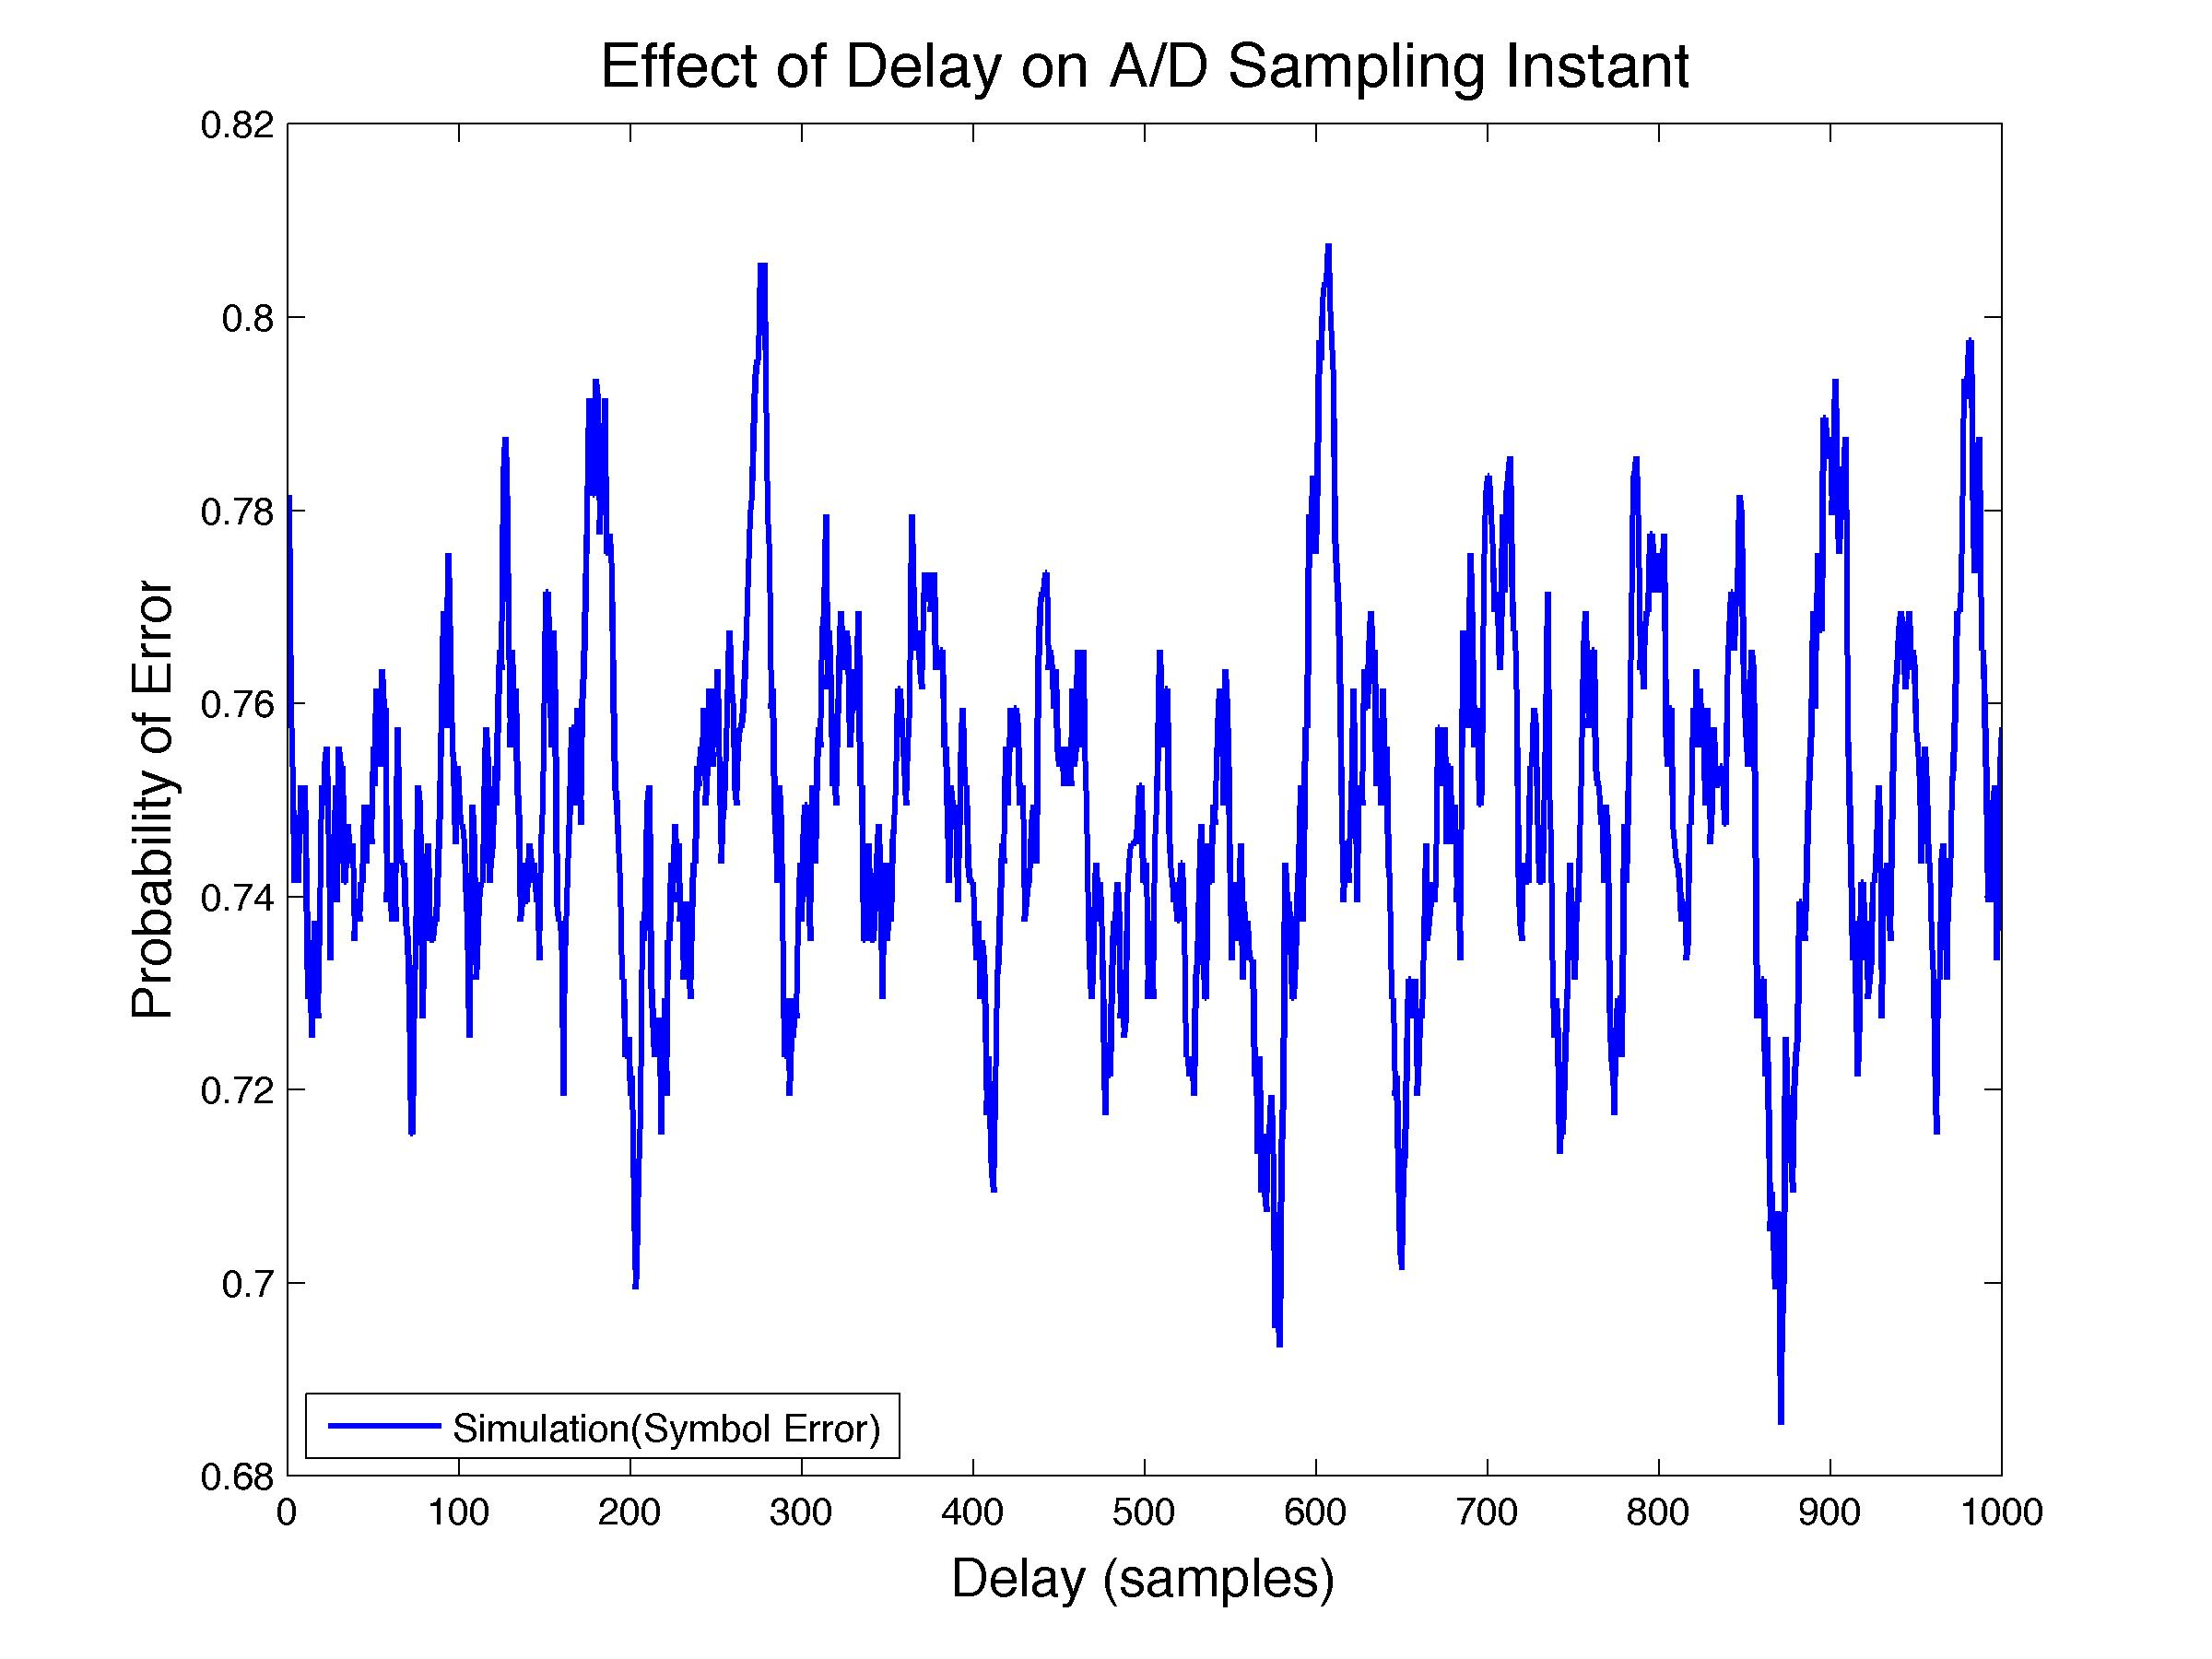
\includegraphics[width=0.7\textwidth]{delaySensitivity.jpg}
\caption{SER plot as a function of delay through the system.  This shows that the system can peform better and worse depending on how in-time the A/D converts.  The effect is not large though. \label{fig:delay}}
\end{figure}

A similar analysis is done for the cutoff frequency of the TX reconstruction filter.   Recall, this filter is in place to bandlimit the DAC output so the high frequency content in the stairs does not create aliases in the lower, passband.  The filter model is controlled by a normalized cutoff frequency, where zero and one are mapped to $\left(0,f_s\right)$.  As such, we expect that the cutoff frequency will not make much difference except if it is way too low.  Even by choosing $f_c$ near one, all frequencies above the sampling frequency will be attenuated and the filter serves its purpose.  However, if $f_c$ gets too low, the information in the waveform may be lost.   \\

\begin{figure}[H]
\centering
\hspace*{-2cm}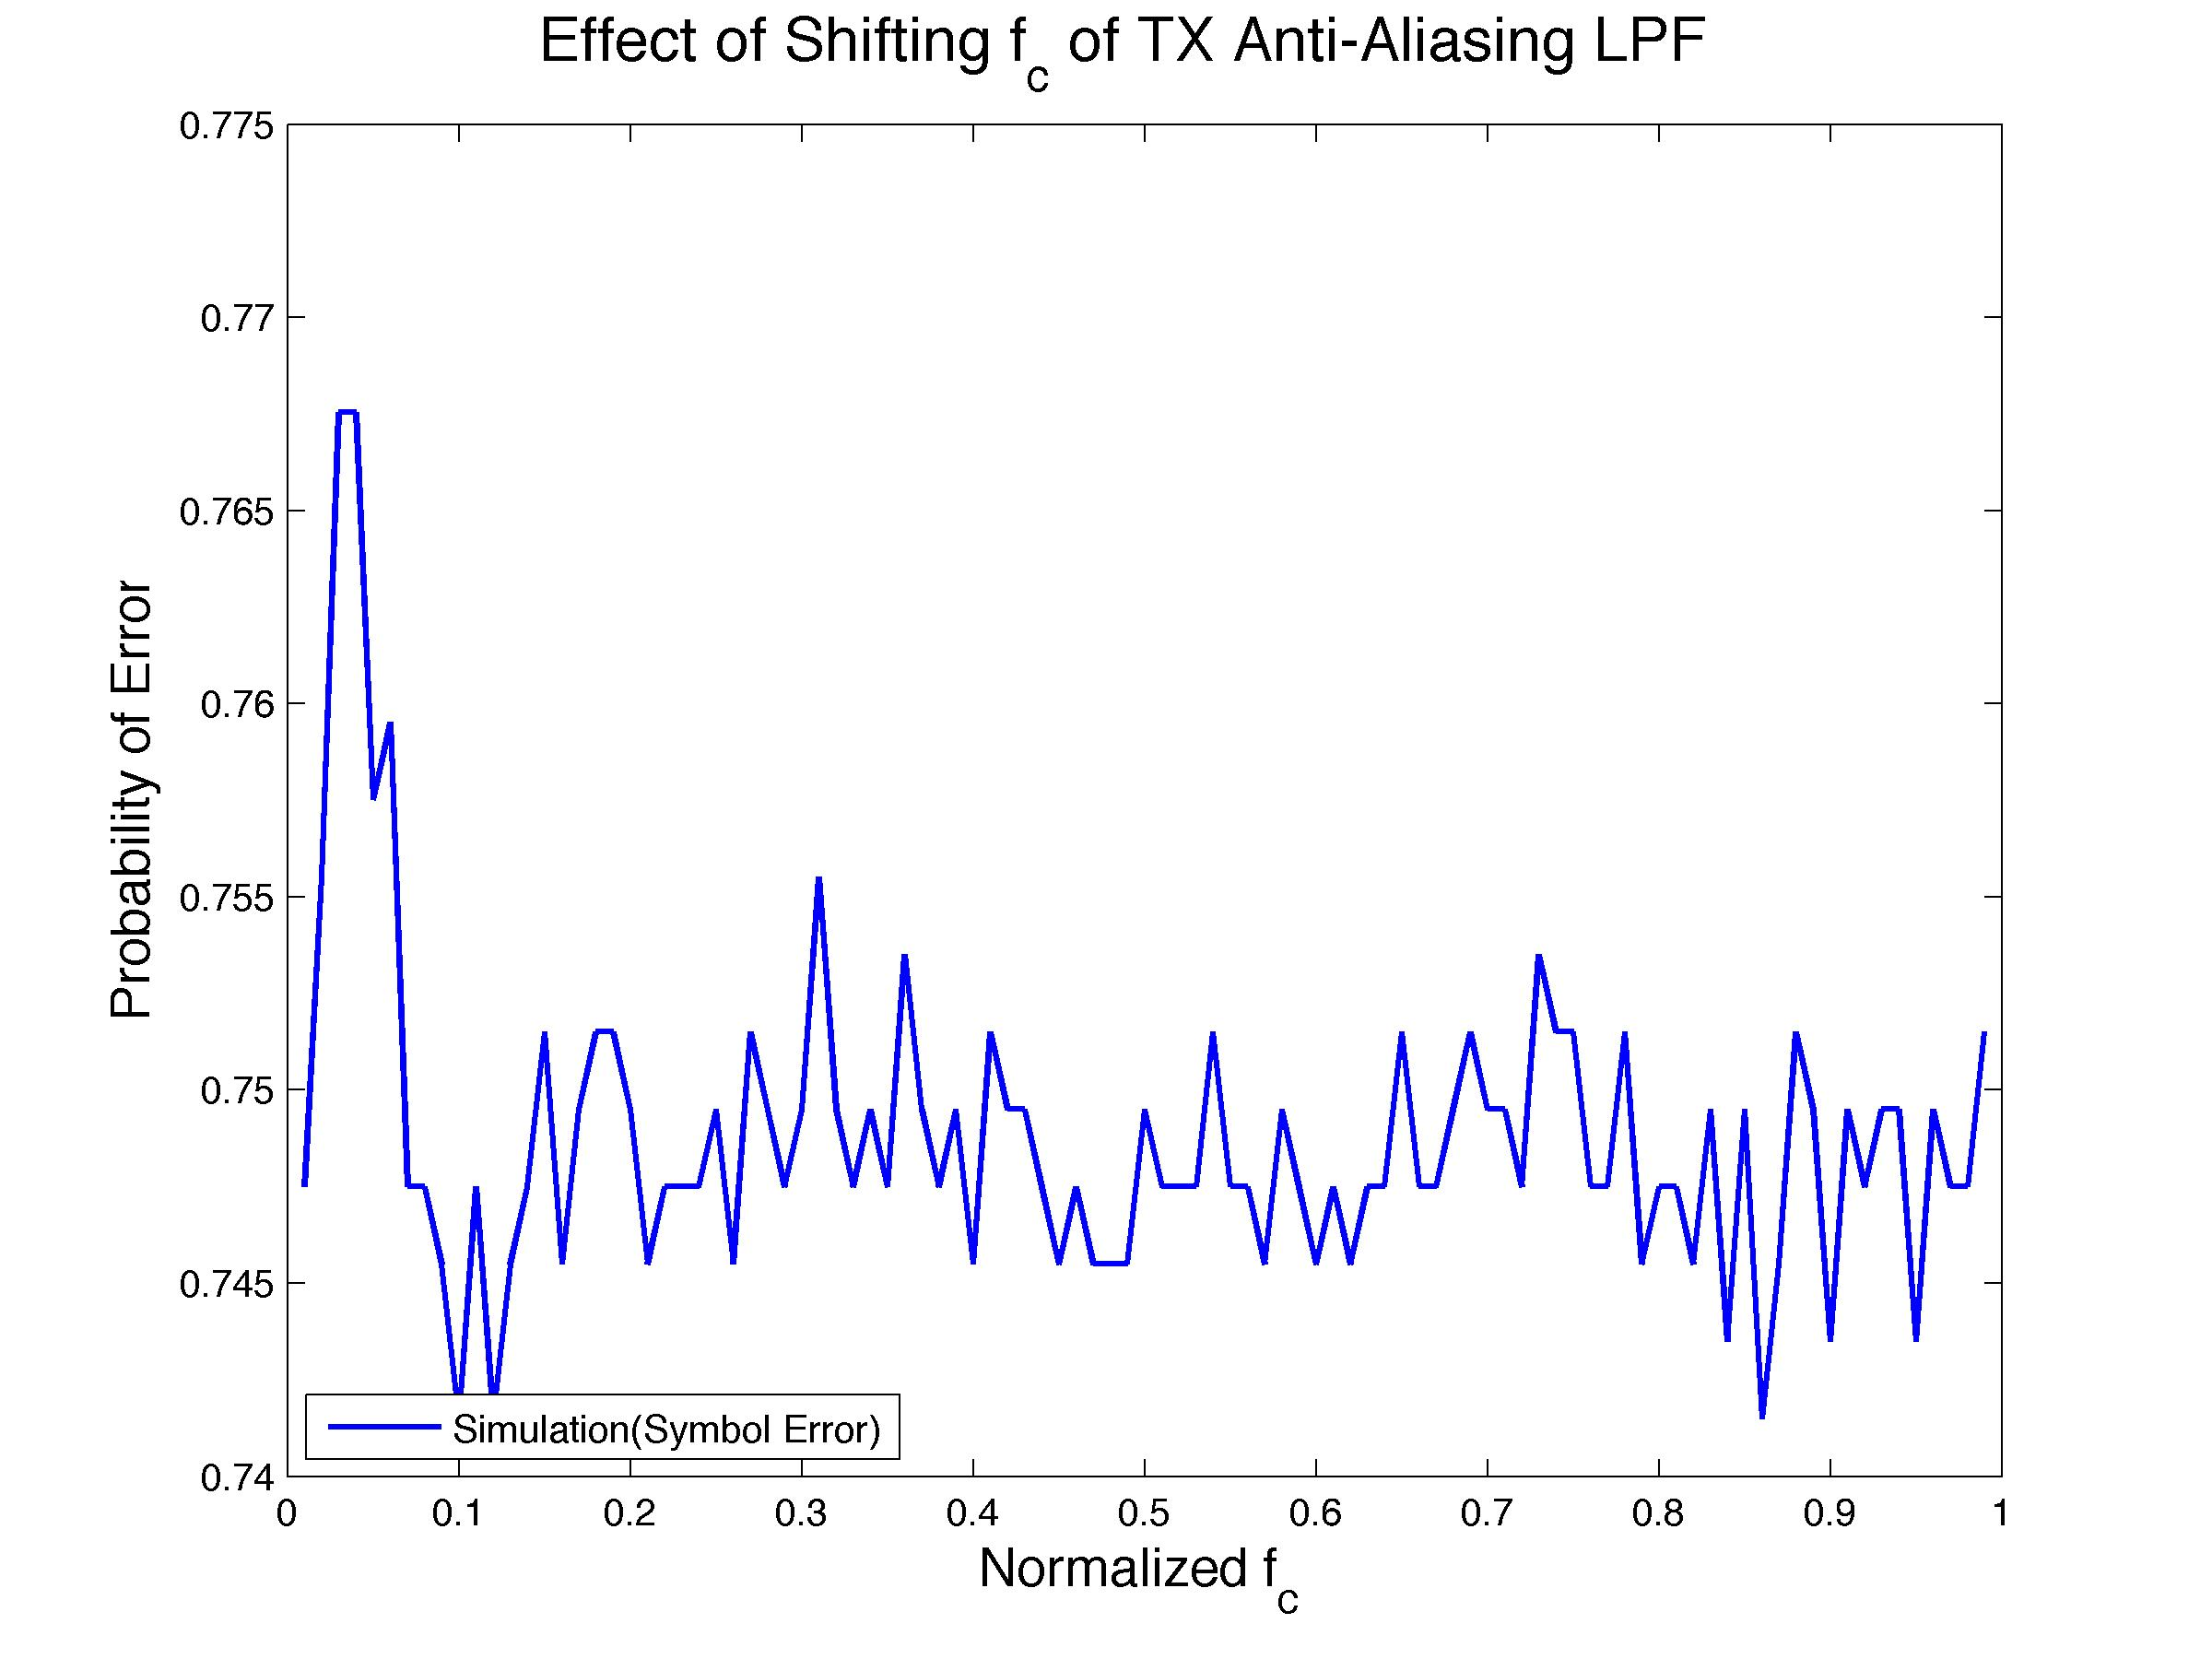
\includegraphics[width=0.7\textwidth]{freqTX.jpg}
\caption{SER plot as a function of cutoff frequency in the TX anti-aliasing Reconstruction filter.  When the cutoff approaches zero, the data is lost. \label{fig:freqTX}}
\end{figure}

Figure~\ref{fig:freqTX} shows the sensitivity analysis of the anti-aliasing LPF normalized cutoff frequency.  The graph confirms the expected behavior discussed above.

\begin{figure}[H]
\centering
\hspace*{-2cm}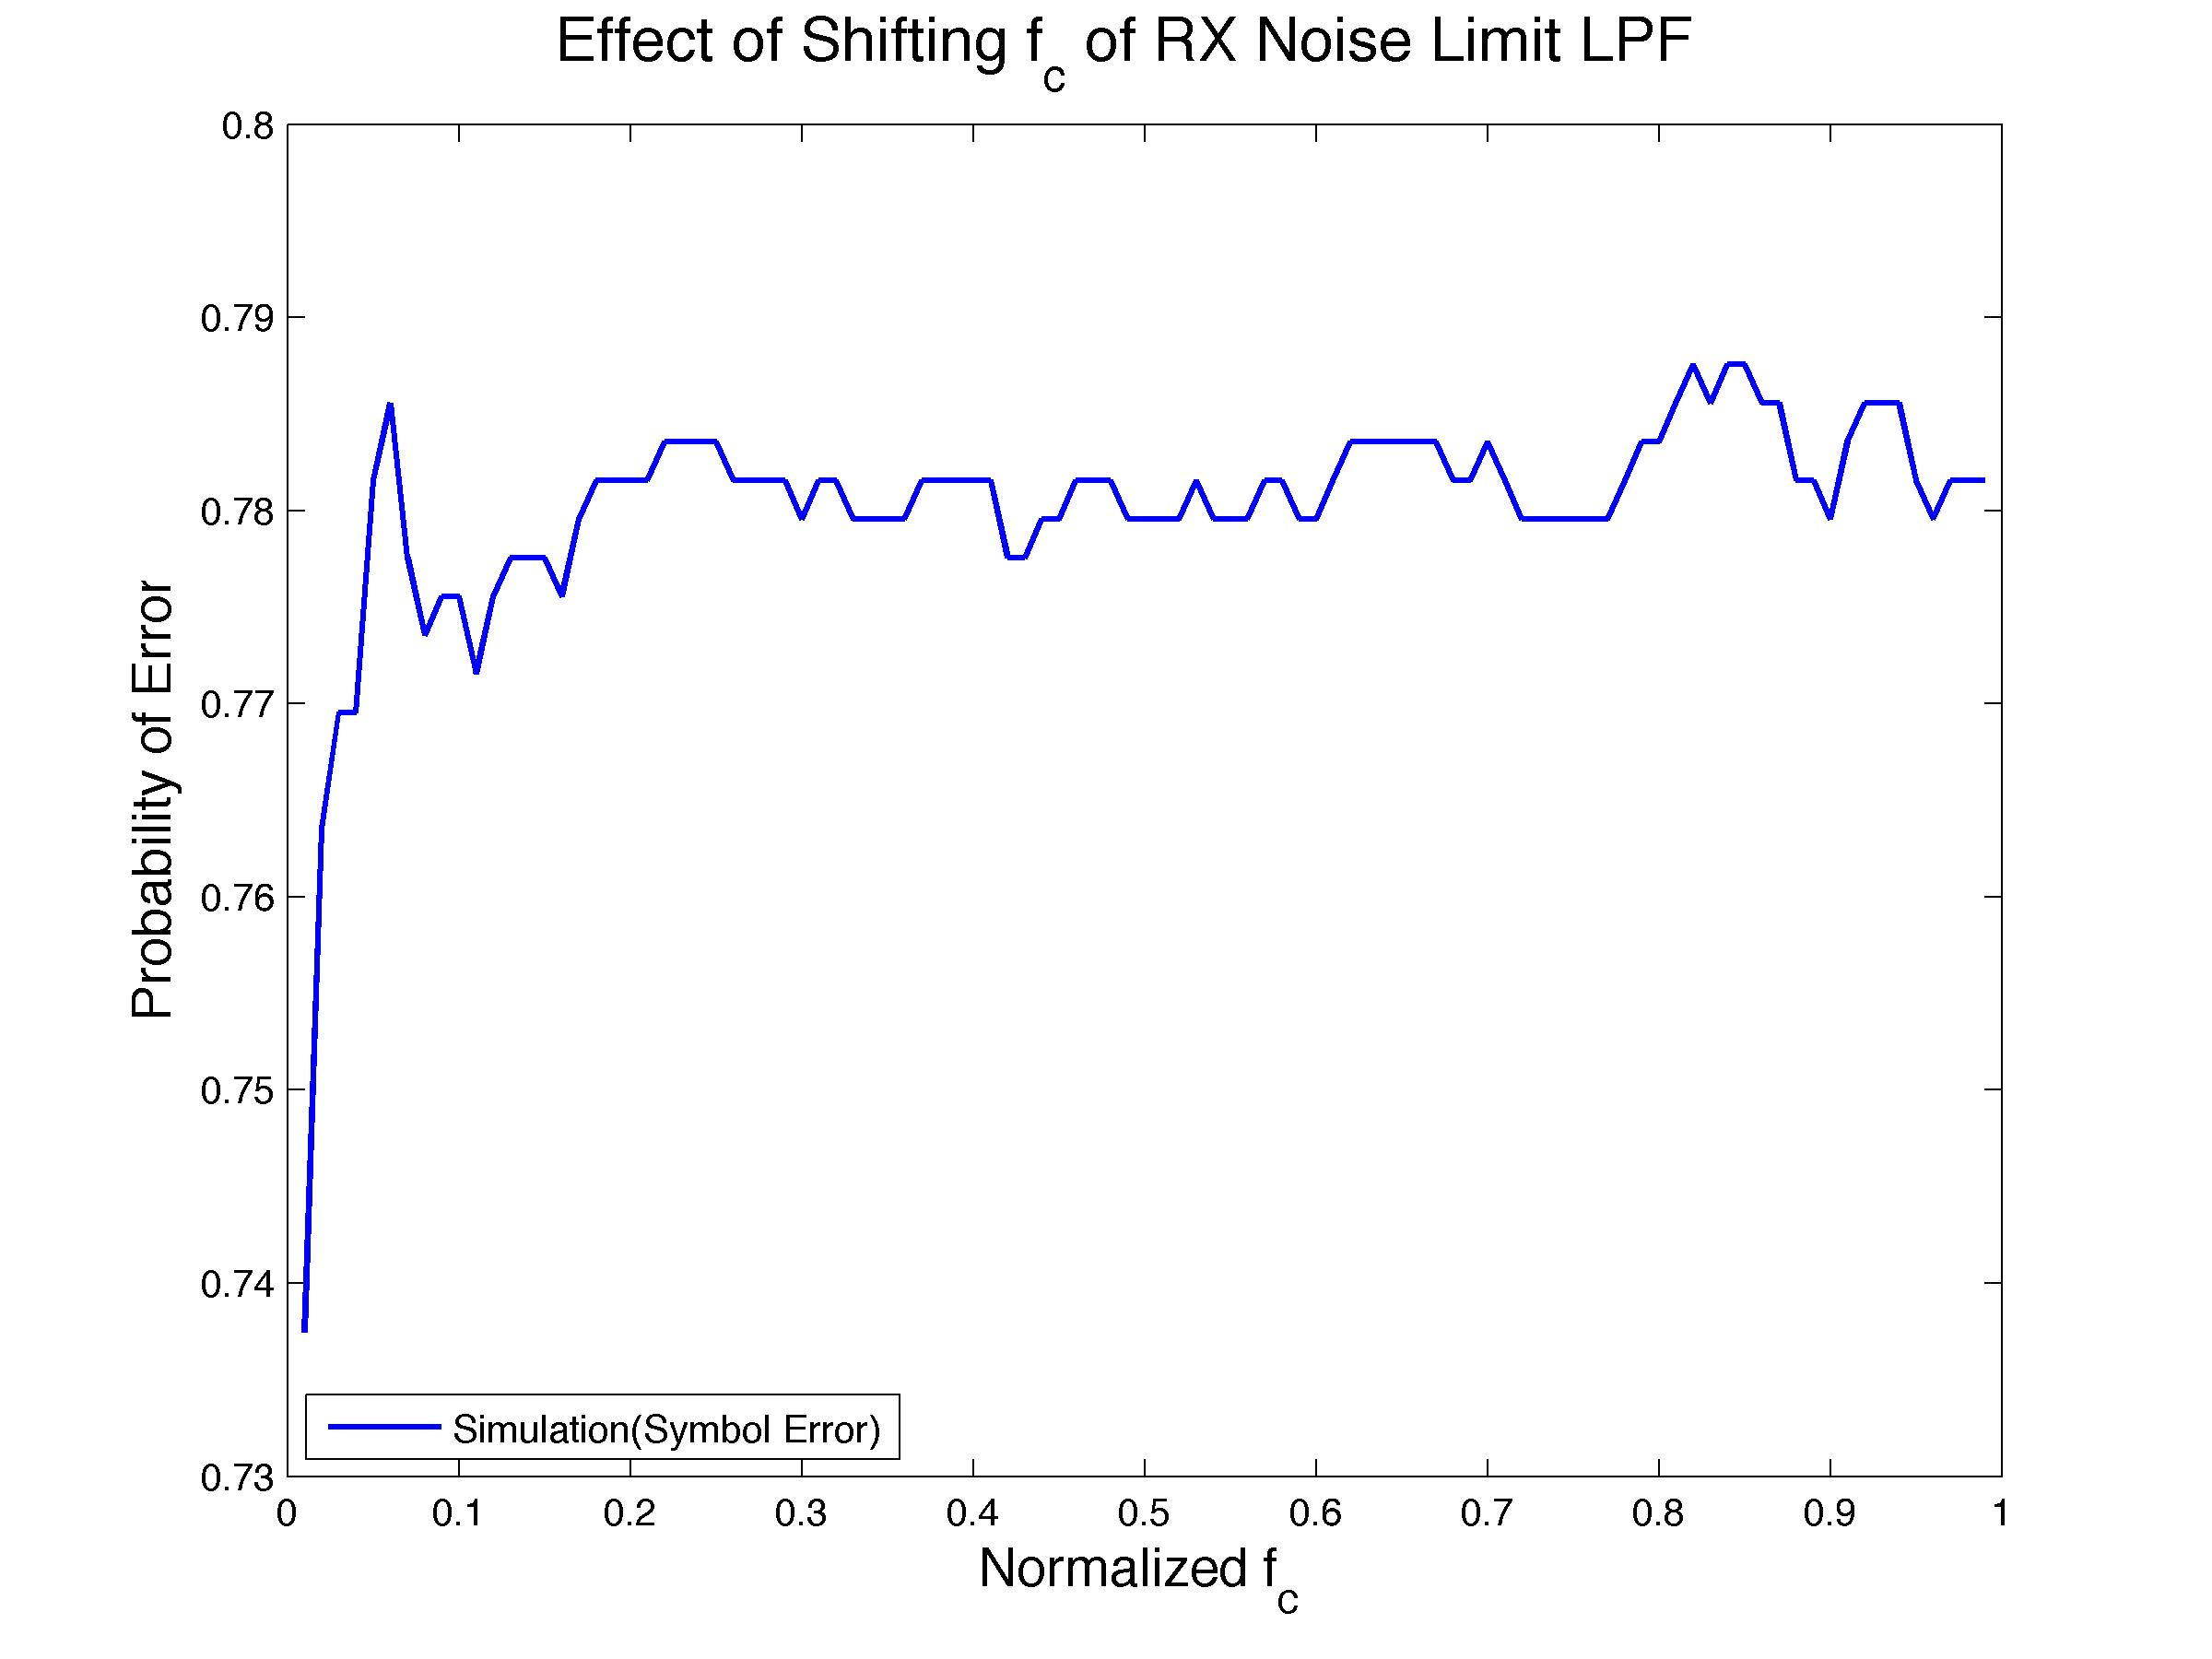
\includegraphics[width=0.7\textwidth]{freqRX.jpg}
\caption{SER plot as a function of cutoff frequency in the RX noise-limiting filter.  When the cutoff is too low, the data transmitted . \label{fig:freqRX}}
\end{figure}

We performed an equivalent analysis on the cutoff frequency in the RX noise-limiting filter.  This filter was aimed to low pass filter the high frequency content from the noise and only allow the signal through.  The same filter model was used, so a similar trend was expected.  The cutoff frequency would always limit the noise with frequency above sampling rate, so the response would mostly look flat.  At near zero cutoff, again we expect none of the data to be transmitted.



\appendix
\newpage
\bibliographystyle{plain}
\bibliography{step4}
\newpage
%% the \\ insures the section title is centered below the phrase: Appendix B
%\section{Project Assignment}
%\label{app:assign}
%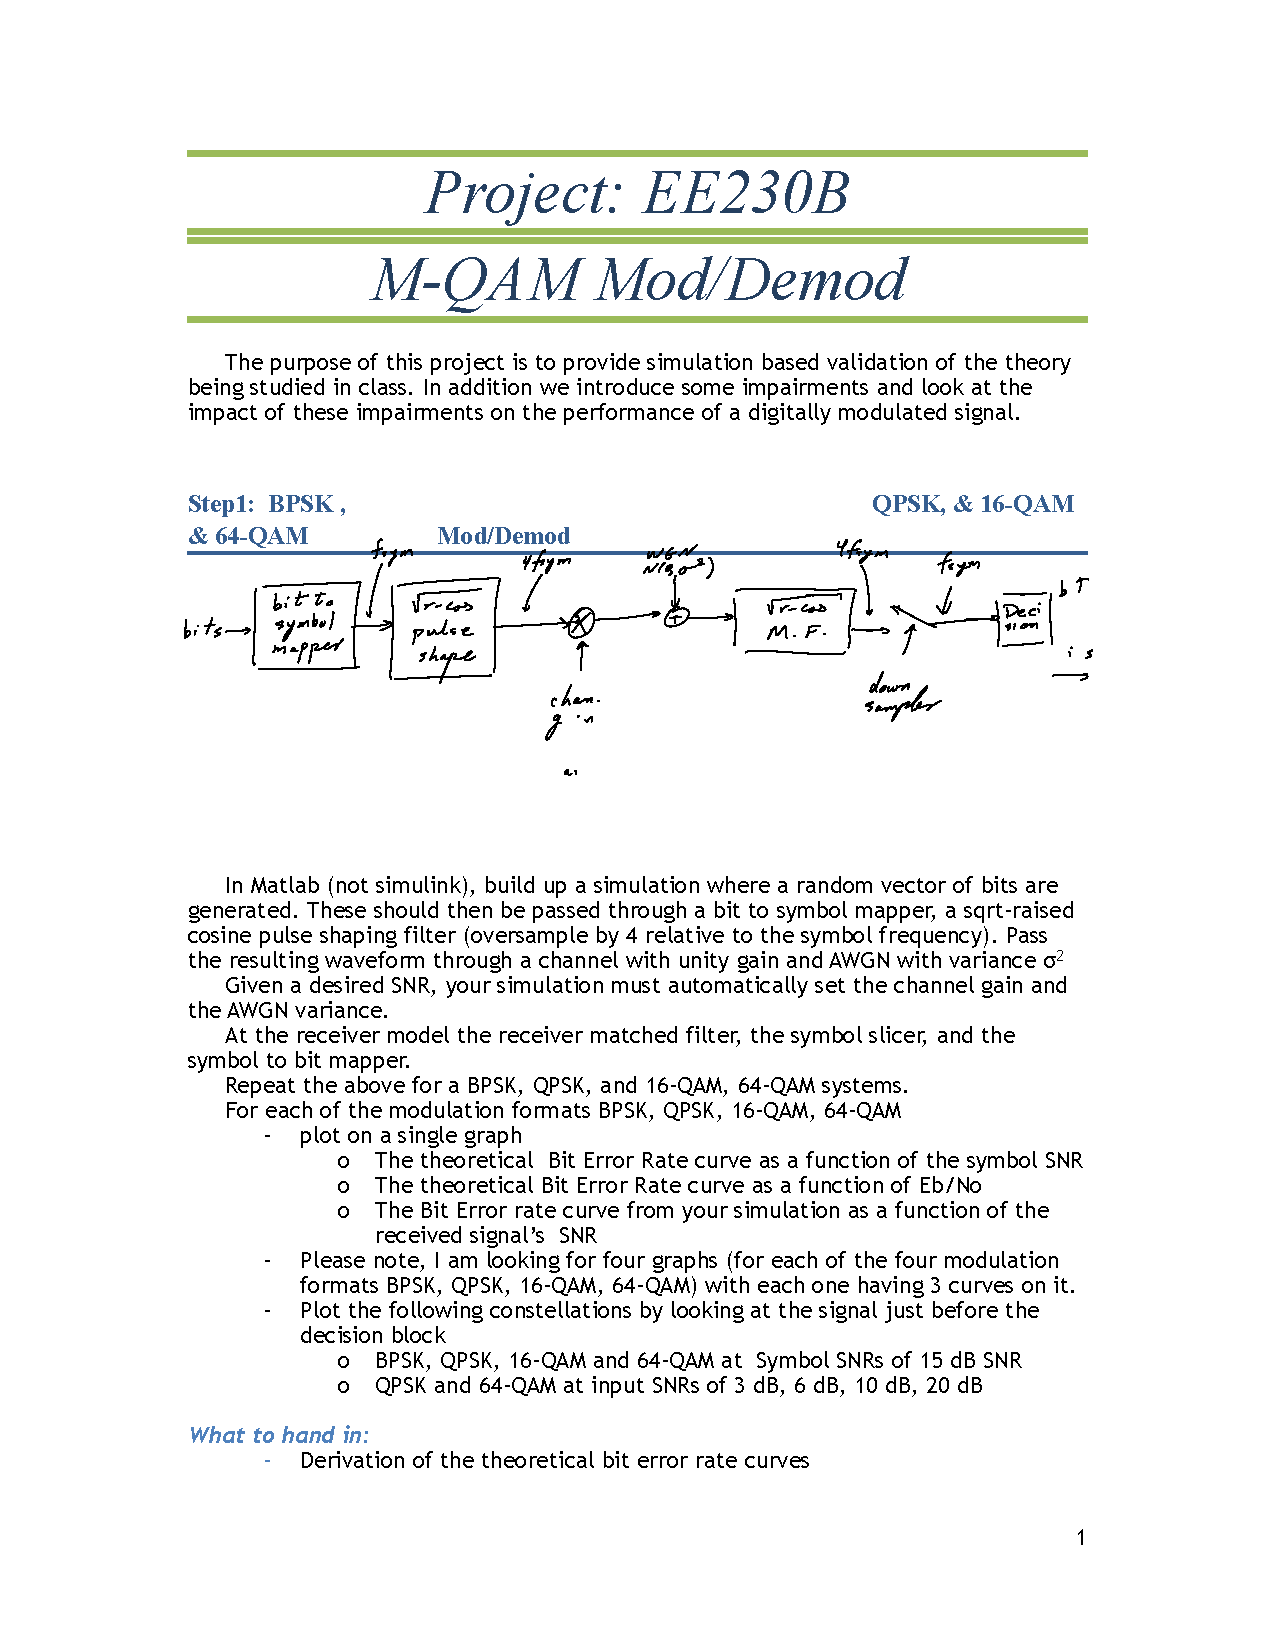
\includepdf[pages={1-5}]{project_overview.pdf}
%\cleardoublepage
%\newpage

\section{Random Bit Sequence Generator}
\label{app:random_bit_generator}
\lstinputlisting{random_bit_generator.m}

\section{Bit to Symbol Mapper}
\label{app:bittosym}
\subsection{QPSK Modulation}
\label{app:qpsk_mod}
\lstinputlisting{qpsk_mod.m}

\section{Up Sampler}
\label{app:impulse_train}
\lstinputlisting{impulse_train.m}

\section{Square Root Raised Cosine Filter}
\label{app:sqrt_raised_cosine}
\lstinputlisting{sqrt_raised_cosine.m}

\section{Additive Gaussian White Noise Channel}
\label{app:awgn_channel}
\lstinputlisting{awgn_complex_channel.m}

\section{Sampler}
\label{app:sampler}
\lstinputlisting{sampler.m}

\section{Decision Block}
\label{app:dblocks}
\subsection{QPSK Demodulation}
\label{app:qpsk_demod}
\lstinputlisting{qpsk_demod.m}

\section{Butterworth Filter}
\label{app:butterworth}
\lstinputlisting{ButterworthFilter.m}

\section{Conversion}
\label{app:convert}
\subsection{Analog-to-Digital Converter}
\label{app:ad}
\lstinputlisting{AD_conv.m}
\subsection{Digital-to-Analog Converter}
\label{app:da}
\lstinputlisting{DA_conv.m}

\subsection{Zero Hold}
\label{app:zero}
\lstinputlisting{ZeroHoldDecimation.m}
\lstinputlisting{ZeroHoldInterpolation.m}

\section{Sensitivity}
\label{app:sensitivity}
\subsection{Setup Code}
\lstinputlisting{qpskSetupFile.m}

\subsection{Delay}
\label{app:delay}
\lstinputlisting{sensitivityDelay.m}

\subsection{TX Filter $f_c$}
\label{app:freqTX}
\lstinputlisting{sensitivityFreqTX.m}

\subsection{RX Filter $f_c$}
\label{app:freqRX}
\lstinputlisting{sensitivityFreqRX.m}


\end{document}